%Version 3 December 2023
% See section 11 of the User Manual for version history
%
%%%%%%%%%%%%%%%%%%%%%%%%%%%%%%%%%%%%%%%%%%%%%%%%%%%%%%%%%%%%%%%%%%%%%%
%%                                                                 %%
%% Please do not use \input{...} to include other tex files.       %%
%% Submit your LaTeX manuscript as one .tex document.              %%
%%                                                                 %%
%% All additional figures and files should be attached             %%
%% separately and not embedded in the \TeX\ document itself.       %%
%%                                                                 %%
%%%%%%%%%%%%%%%%%%%%%%%%%%%%%%%%%%%%%%%%%%%%%%%%%%%%%%%%%%%%%%%%%%%%%

%%\documentclass[referee,sn-basic]{sn-jnl}% referee option is meant for double line spacing

%%=======================================================%%
%% to print line numbers in the margin use lineno option %%
%%=======================================================%%

%%\documentclass[lineno,sn-basic]{sn-jnl}% Basic Springer Nature Reference Style/Chemistry Reference Style

%%======================================================%%
%% to compile with pdflatex/xelatex use pdflatex option %%
%%======================================================%%

%%\documentclass[pdflatex,sn-basic]{sn-jnl}% Basic Springer Nature Reference Style/Chemistry Reference Style


%%Note: the following reference styles support Namedate and Numbered referencing. By default the style follows the most common style. To switch between the options you can add or remove “Numbered” in the optional parenthesis. 
%%The option is available for: sn-basic.bst, sn-vancouver.bst, sn-chicago.bst%  
 
%%\documentclass[pdflatex,sn-nature]{sn-jnl}% Style for submissions to Nature Portfolio journals
%%\documentclass[pdflatex,sn-basic]{sn-jnl}% Basic Springer Nature Reference Style/Chemistry Reference Style
%%\documentclass[pdflatex,sn-mathphys-num]{sn-jnl}% Math and Physical Sciences Numbered Reference Style 
%%\documentclass[pdflatex,sn-mathphys-ay]{sn-jnl}% Math and Physical Sciences Author Year Reference Style
%%\documentclass[pdflatex,sn-aps]{sn-jnl}% American Physical Society (APS) Reference Style
\documentclass[pdflatex,sn-vancouver,Numbered]{bst/sn-jnl}% Vancouver Reference Style
%%\documentclass[pdflatex,sn-apa]{sn-jnl}% APA Reference Style 
%%\documentclass[pdflatex,sn-chicago]{sn-jnl}% Chicago-based Humanities Reference Style


%%%% Standard Packages
%%<additional latex packages if required can be included here>

\usepackage{graphicx}%
\usepackage{multirow}%
\usepackage{amsmath,amssymb,amsfonts}%
\usepackage{amsthm}%
\usepackage{mathrsfs}%
\usepackage[title]{appendix}%
\usepackage{xcolor}%
\usepackage{textcomp}%
\usepackage{manyfoot}%
\usepackage{booktabs}%
\usepackage{algorithm}%
\usepackage{algorithmicx}%
\usepackage{algpseudocode}%
\usepackage{listings}%
\usepackage{booktabs}
\usepackage[graphicx]{realboxes}
\usepackage{graphicx}
\usepackage{adjustbox}
\usepackage{subcaption}
\usepackage{nameref}
\usepackage{verbatim}

%%%%

%%%%%=============================================================================%%%%
%%%%  Remarks: This template is provided to aid authors with the preparation
%%%%  of original research articles intended for submission to journals published 
%%%%  by Springer Nature. The guidance has been prepared in partnership with 
%%%%  production teams to conform to Springer Nature technical requirements. 
%%%%  Editorial and presentation requirements differ among journal portfolios and 
%%%%  research disciplines. You may find sections in this template are irrelevant 
%%%%  to your work and are empowered to omit any such section if allowed by the 
%%%%  journal you intend to submit to. The submission guidelines and policies 
%%%%  of the journal take precedence. A detailed User Manual is available in the 
%%%%  template package for technical guidance.
%%%%%=============================================================================%%%%

%% as per the requirement new theorem styles can be included as shown below
\theoremstyle{thmstyleone}%
\newtheorem{theorem}{Theorem}%  meant for continuous numbers
%%\newtheorem{theorem}{Theorem}[section]% meant for sectionwise numbers
%% optional argument [theorem] produces theorem numbering sequence instead of independent numbers for Proposition
\newtheorem{proposition}[theorem]{Proposition}% 
%%\newtheorem{proposition}{Proposition}% to get separate numbers for theorem and proposition etc.

\theoremstyle{thmstyletwo}%
\newtheorem{example}{Example}%
\newtheorem{remark}{Remark}%

\theoremstyle{thmstylethree}%
\newtheorem{definition}{Definition}%

\raggedbottom
%%\unnumbered% uncomment this for unnumbered level heads

% Macro: \dself{<mean>}{<std>}
\newcommand{\dself}[2]{$d_{\text{self}} = #1 \pm #2$}

% Macro: \dref{<mean>}{<std>}
\newcommand{\dref}[2]{$d_{\text{ref}} = #1 \pm #2$}

% Macro: \dselfdref{df}{tvalue}{pvalue}
% Exact p-value
\newcommand{\dselfdrefp}[3]{$d_{\text{self}} < d_{\text{ref}},\ \text{Welch's } t(#1) = #2,\ p = #3$}

% p-value as an upper bound
\newcommand{\dselfdrefpl}[3]{$d_{\text{self}} < d_{\text{ref}},\ \text{Welch's } t(#1) = #2,\ p < #3$}

%%%%%%%%%% Macro for lazy stuffs
\newcommand{\totalN}{N = 1086}   % total observations

\begin{document}

\title[Article Title]{Regularity of life rhythms}

%%=============================================================%%
%% GivenName	-> \fnm{Joergen W.}
%% Particle	-> \spfx{van der} -> surname prefix
%% FamilyName	-> \sur{Ploeg}
%% Suffix	-> \sfx{IV}
%% \author*[1,2]{\fnm{Joergen W.} \spfx{van der} \sur{Ploeg} 
%%  \sfx{IV}}\email{iauthor@gmail.com}
%%=============================================================%%

\author*[1]{\fnm{Nguyen} \sur{Luong}}\email{nguyen.luong@aalto.fi}


\author[1]{\fnm{Talayeh} \sur{Aledavood}}\email{talayeh.aledavood@aalto.fi}


\affil*[1]{\orgdiv{Computer Science}, \orgname{Aalto University} \city{Espoo}, \country{Finland}}

%%==================================%%
%% Sample for unstructured abstract %%
%%==================================%%

\abstract{Humans organize their daily lives around a constrained set of recurring behavioural patterns, yet the extent to which these routines persist across time, contexts, and populations remains poorly understood. Leveraging multimodal digital traces from smartphones and wearables collected in three large-scale longitudinal studies (\totalN~participants, ), we introduced a framework to quantify individual routine signatures — a concept capturing how individuals allocate their time and transition between distinct latent behavioural states. We find that these signatures are highly distinctive and remain stable over weeks and months.}

\keywords{}

\maketitle

\section{Introduction}\label{sec1}

Humans’ daily lives are inherently synchronized with the 24-hour day–night cycle. This circadian rhythm shapes essential physiological and behavioural routines—such as sleep, physical activity, communication, and mobility. 
%Maintaining the regularity of these routines are important for health, supporting well-being \cite{heintzelman2019routines}, enhancing life satisfaction \cite{margraf2016social}, and ensuring good sleep quality \cite{carney2006daily}. 
Daily routines are naturally stable, as individuals structure their activities to meet social, occupational, and environmental demands \cite{monk1994regularity}. This persistence has been documented through structured surveys and diaries, which consistently revealed predictable temporal patterns (e.g., meal times, sleep schedules) and spatial regularities (e.g., commuting routes) \cite{hansonSystematicVariabilityRepetitiouTesserae988a, monk1990social, soehnerCircadianPreferenceSleepWake2011}. In modern times, the emerging ubiquity of personal digital devices has enabled large-scale, longitudinal analyses of human behaviour, confirming these findings with much higher resolution and longer observation period. For instance, studies using GPS and call-record data also demonstrate that human's mobility follows highly predictable spatiotemporal trajectories, with individuals visiting a limited set of familiar locations in stable sequences \cite{songLimitsPredictabilityHuman2010, song2010modelling, alessandretti2020scales}. Similarly, individual's communication patterns display distinctive and persistent structures. Saramaki et al. conceptualized this structure as the social signature \cite{saramaki2014persistence}—the characteristic way individuals distribute communication effort across contacts. These signatures are found in different communication means (calls, SMS, emails) and remain robust despite substantial turnover in individual's social networks \cite{saramaki2014persistence, aledavoodDailyRhythmsMobile2015a, heydari2018multichannel, loriteLongTermEvolutionEmail2016}. Routine persistence extends from the physical world to the digital world, with high individual-level predictability observed in the timing and frequency of web visits \cite{barbosa2016returners, hu2018life, kulshrestha2021web} as well as in app usage patterns \cite{malmi2016you, kosinski2013private, petersSocialMediaUse2024, shawBehavioralConsistencyDigital2022}. 

Despite this evidence, there are still important gaps. First, most studies examined single behavioural domains in isolation, leaving it unclear whether persistence is an intrinsic, person-specific property that generalizes to multifaceted daily routines integrating sleep, activity, communication, and mobility. Second, if human's routine are indeed stable and distinctive, the extent of re-identification risk they pose— has not been systematically quantified. 


\begin{comment}
Latent structure approaches—eigenbehaviours \cite{eagleEigenbehaviorsIdentifyingStructure2009a}, activity/mobility classes \cite{jiangClusteringDailyPatternMoMo-Mood012, yangIdentifyingLatentActivity2023a}, and decompositions such as NMF and LDA \cite{aledavood2022quantifying, girardiniAdaptationStudentBehavioural2023a, farrahiDiscoveringRoutinesLargescale2011, farrahiWhatDidYou2008}, as well as clustering \cite{kasDigitalBehaviouralSignatureMoMo-Mood024, zhou2022predicting, yan2025relapse}—reveal coherent daily patterns, but prior studies have not systematically quantified how these latent routines persist as person-specific signatures, nor how persistence varies across populations and environments.
\end{comment}

In this work, we introduce an approach for quantifying the persistence of multifaceted daily routines. Using Gaussian Mixture Model (GMM), we model each individual’s daily behaviour as a mixture of Gaussian latent routine classes, capturing recurring patterns across domains such as sleep, activity, and device usage. Building on the concept of the social signature, we define the resulting distribution over these latent routines as a routine signature, representing how individuals allocate time across behavioural patterns. We further introduce the transition signature, which captures the stability of day-to-day transitions between different routine types. Finally, using individual cluster of routine and their transition, we examine the degree of re-identification.

Using behavioural data from three studies, we examined the persistence of routine signatures and investigated how these signatures can be traced back to the individual. Across populations, we found that individuals exhibit stable and distinctive routine signatures, reflected both in how they allocate their time and how they transitioned between routines. These patterns are more consistent within individuals than between individuals and remain robust across month-long observation periods, but disappeared when there is a long time gap between two consecutive observation windows. 

\section*{Results}\label{sec:results}  

\subsection*{Routine cluster characteristics}\label{sec:results:cluster}

Daily routines were quantified across three behavioral domains: device use, physical activity, and sleep. Behaviors were summarized by timing in four daily segments (morning, afternoon, evening, night) and by total daily duration (e.g., total screen time), yielding a 16-dimensional representation for each day (Methods). Using data from \totalN participants and over 153,000 person-days across three studies, we applied unsupervised clustering to each study to identify latent patterns of daily behavior (z-scored per participtants to focus on individual variability). For each study, the optimal cluster number was determined from model fit indices and the average Bhattycharya distance between clusters - higher distance suggest more better clusters separation (see \nameref{sec:methods}). Model selection favored a full-covariance GMM with optimal component counts of 8, 11, and 8 for Tesserae-GLOBEM. Given the marginal improvement for K=11 in MoMo-Mood, we proceeded with K=8 for all studies.

\begin{figure}[htbp!]
    \centering
    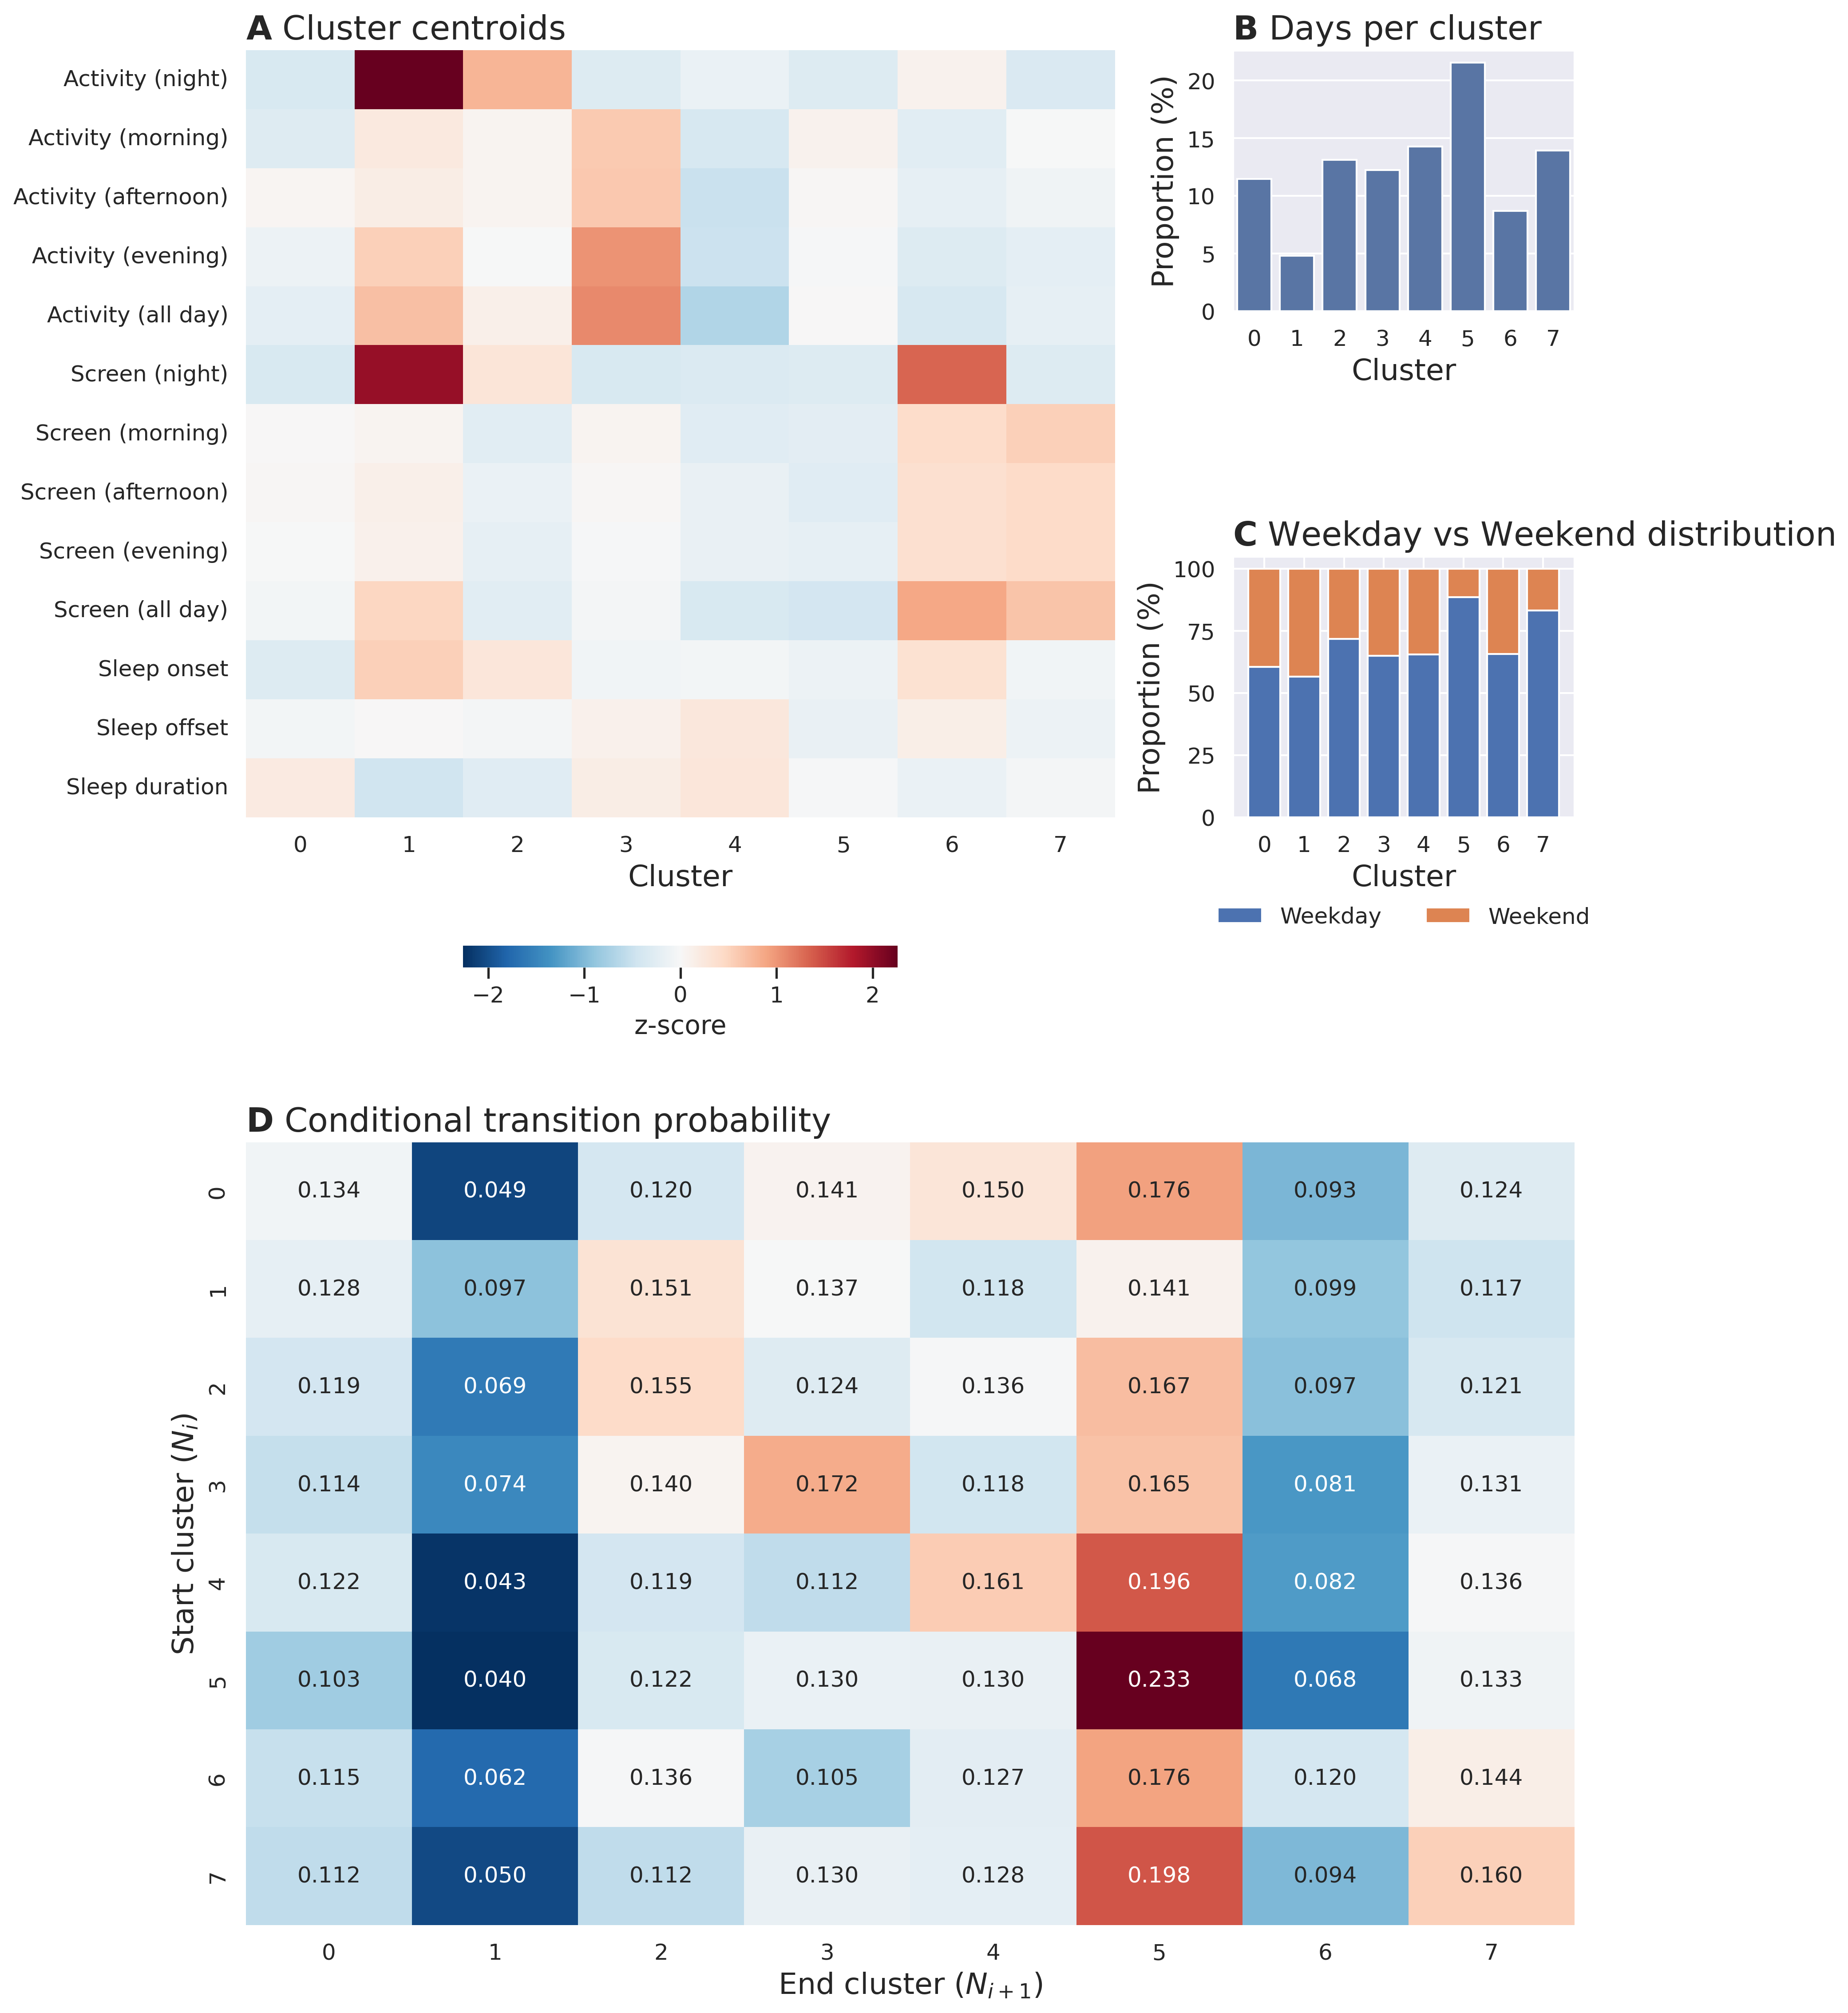
\includegraphics[width=1\linewidth]{figures/tesserae_summary.png}
    \caption{Cluster summary for Tesserae. (A) Cluster centroids: Heatmap showing the average standardized feature values (z-scores) for each behavioral feature within each cluster. Each feature’s z-score is computed per individual to reflect within-person deviations. Higher (red) and lower (blue) values represent positive and negative deviations from an individual’s mean, respectively. (B) Days per cluster: Histogram showing the distribution of all recorded days across clusters, aggregated across the study population. (C) Weekday–weekend distribution: Stacked bar plot depicting the proportion of weekdays (blue) and weekends (orange) within each cluster. Certain clusters exhibit a significant weekend skew, depicting leisure-oriented behaviours that emerge on non-working days. (D) Heatmap of adjacency matrix depicting the conditional transition probability between cluster pairs. Transition probabilities are computed and normalized per participant, then averaged across participants to obtain a population means. Higher values indicate more frequent transitions.}
    \label{fig:tesserae-cluster-summary}
\end{figure}

In Tesserae, a total of 592 participants and 106172 person-days were included in this analysis. The cluster profiles (centroids) are shown in \autoref{fig:tesserae-cluster-summary}A, with each cell showing the deviations from individual baseline.  One dominant cluster presented the most typical routine (see \autoref{fig:tesserae-cluster-summary}B, characterized by all features sitting near the mean level and a small dip in screen usage. This cluster represents a typical workday of the white-collar cohort. As shown in \autoref{fig:tesserae-cluster-summary}C, some smaller clusters emerged, depicting possible weekend or holiday patterns. They were characterized by slight increase in screen usage and sleep duration (Cluster 4), or a large increase in nightly physical activity (Cluster 6). It is worth noting that the organic weekend naturally arise from the observations, given that temporal information was not provided during model fit. Clusters characteristics of MoMo-Mood and GLOBEM are presented in Appendix 2.

To assess whether individuals tend to adhere to a single routine or frequently shift between different routine types, we analyzed the transition probabilities between clusters. For each participant, we constructed a transition matrix \(P\) by counting the number of transitions from cluster \(i\) to cluster \(j\), then normalizing each row so that the probabilities sum to 1 (see \nameref{sec:methods}). Each cell \(P_{ij}\) represents the probability of transitioning from routine \(i\) to routine \(j\), with larger values indicating more frequent transitions. If individuals were strongly adapted to a specific routine, we would expect the diagonal entries \(P_{ii}\) - denoting self-transitions - to have the highest values. However, this was not the case. As shown in \autoref{fig:tesserae-cluster-summary}D, most routine clusters converged toward a dominant cluster. The transition probabilities were also diffuse and asymmetric, indicating that the likelihood of moving between clusters varies across individuals. We repeated the analysis on MoMo-Mood and GLOBEM and observed similar results, suggesting that these properties of routine transitions are consistent across different populations.


\subsection*{Persistence of individual's routine signature} \label{sec:results:signature_persistence}

For each participant and time segment, a \textit{routine signature} is defined as the vector of cluster proportions, sorted in descending order of frequency within that segment (\nameref{sec:methods}). We examined whether an individual’s routine is more similar to their own than to others’ by comparing the distributions of within-person distances \(d_{\text{self}}\) and between-person reference distances \(d_{\text{ref}}\) (see \autoref{fig:dself_dref}). For each participant \(i\), \(d_{\text{ref},i}\) was computed as the mean distance between \(i\)’s routine signature and those of all other participants, matched by time segment.

In Tesserae and MoMo-Mood, we retained participants with at least 270 days of data and divided them into two equal windows (135 days each). In GLOBEM, we included participants who participated in at least two consecutive study waves. For GLOBEM, the reference distance \(d_{\text{ref}}\) was computed by comparing the routine signature of individual \(i\) between waves \(j\) and \(j+1\) against the signatures of all other participants in the same waves.

Despite variability in total activity levels, individuals tended to allocate a large proportion of their time to a small number of routines, with the top two routine accounting for $(57.63 \pm 11.43)\%$ of total daily behaviour across all studies. This individuality was evident in the clear separation between participants’ signatures, even when observed months apart. In Tesserae (\(N=148\)), we observed strong persistence of routine signatures. Using JSD as distance metric, within-person distances were substantially smaller than between-person distances \dself{0.135}{0.041} vs. \dref{0.164}{0.026} (\dselfdrefpl{226.03}{-8.49}{10^{-3}}), indicating that individuals maintained highly distinctive routine patterns across time. A sanity check using cosine distance produced similar results, with \dself{0.031}{0.021} and \dref{0.055}{0.013} (\dselfdrefpl{246.83}{-11.69}{10^{-3}}). 

In MoMo-Mood (\(N=15\)), the patterns were similar despite the smaller sample size. Routine signatures again showed strong persistence, with JSD distances of \dself{0.164}{0.026} vs. \dref{0.222}{0.075} (\dselfdrefpl{29.99}{-12.13}{10^{-3}}). Robustness check using cosine distances also produced comparable results, with \dself{0.027}{0.026} and \dref{0.096}{0.035} (\dselfdrefp{27.8}{-6.21}{< 10^{-3}}).

In both studies, further sensitivity checks using a smaller threshold and window (180 days - 60-day windows) revealed similar results. 

In contrast, results from GLOBEM (\(N=125\)) revealed a different finding. Here, individuals exhibited larger within-person distances than in other studies (JSD: \dself{0.253}{0.107}), and these values were not significantly different from the average reference distance \dref{0.248}{0.035} (\dselfdrefp{40.63}{0.28}{0.783}). This indicates that, unlike in Tesserae and MoMo-Mood, routine signatures in GLOBEM lacked persistence, and individuals could not be reliably distinguished from one another based on their time allocation patterns.

\begin{comment}
We further examined routine signatures by ignoring rank order and treating them purely as distributions of time allocation across routines. Under this formulation, the results remained consistent: \dself{0.232}{0.071} and \dref{0.360}{0.059} (\dselfdrefpl{258.42}{-16.86}{10^{-3}}). Notably, the $d_{self}$ values were larger in this case, suggesting that removing rank information reduces within-person similarity.
\end{comment}

\begin{figure}
    \centering
    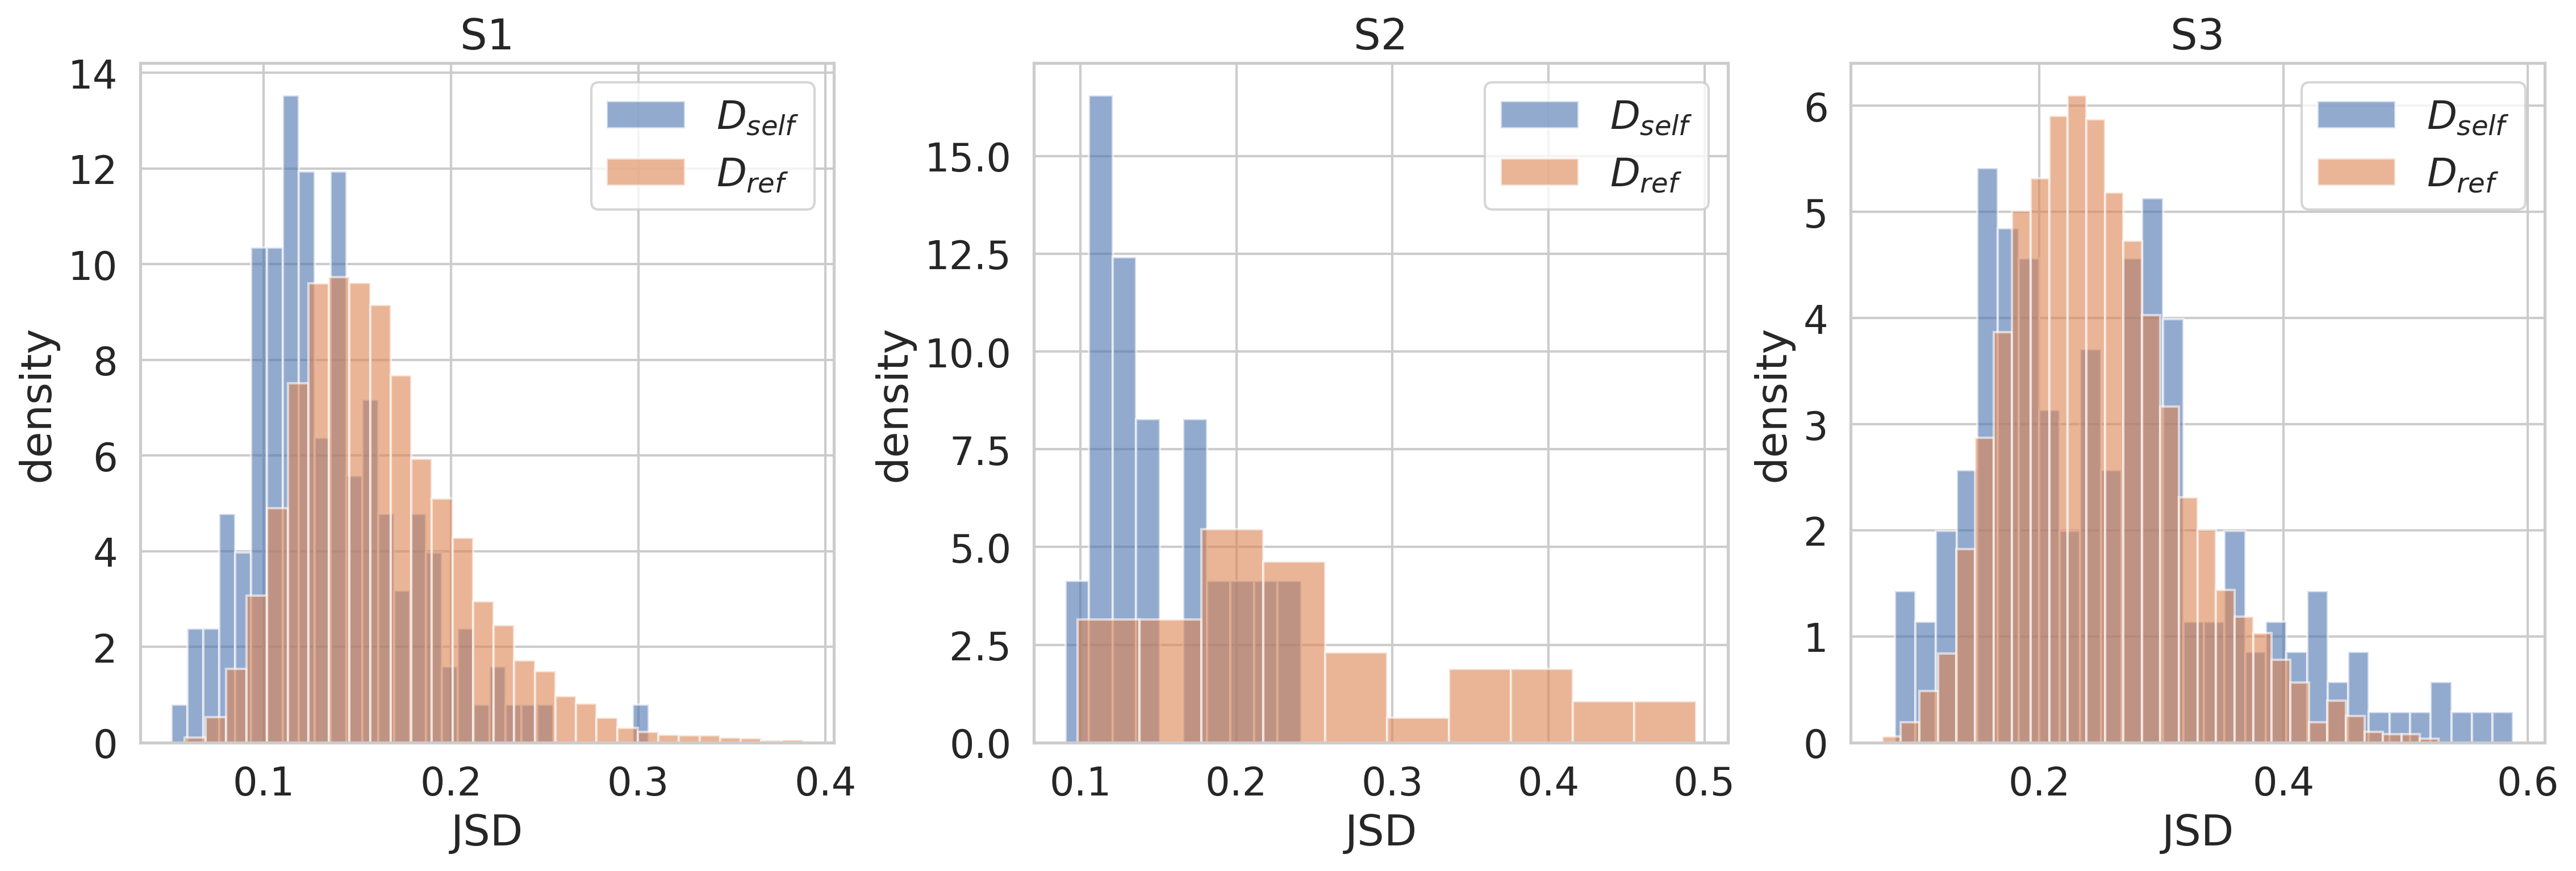
\includegraphics[width=1\linewidth]{figures/combined_dself_dref_ranked_jsd.png}
    \caption{Self-distance and reference-distance of routine signature across studies.}
    \label{fig:dself_dref}
\end{figure}

\subsection*{Transition between routines exhibits similar persistence}

Beyond individual-specific time allocation across routines, we hypothesized that each person’s transition dynamics between routines was also distinctive. In other words, people do not follow the same routine every day but instead switch between different latent routine clusters over time in unique ways. For example, one individual may frequently alternate between workday and weekend routines with minimal variability, whereas another may display irregular transitions across several distinct routine types.

To test this hypothesis, we first constructed a transition probability matrix 
\(\mathbf{P} \in \mathbb{R}^{K \times K}\) for each participant and segment, 
where \(K\) is the number of routine clusters. We define the transition signature of an individual as the mean row-wise 
distance between their transition matrices across consecutive segments: 
\(d_{\mathrm{self}} = 
D(\mathbf{P}^1, \mathbf{P}^{2}) \). Similarly, the reference distance of individual $i$ was computed by calculating the distance between each participant’s transition matrix with those of all other participants in the same segment, then averaged across 
segments: 
\(d_{\mathrm{ref}} = \frac{1}{2} (
D(\mathbf{P_i}^1, \mathbf{P_j}^{1}) + D(\mathbf{P_i}^2, \mathbf{P_j}^{2}))\)

\begin{figure}
    \centering
    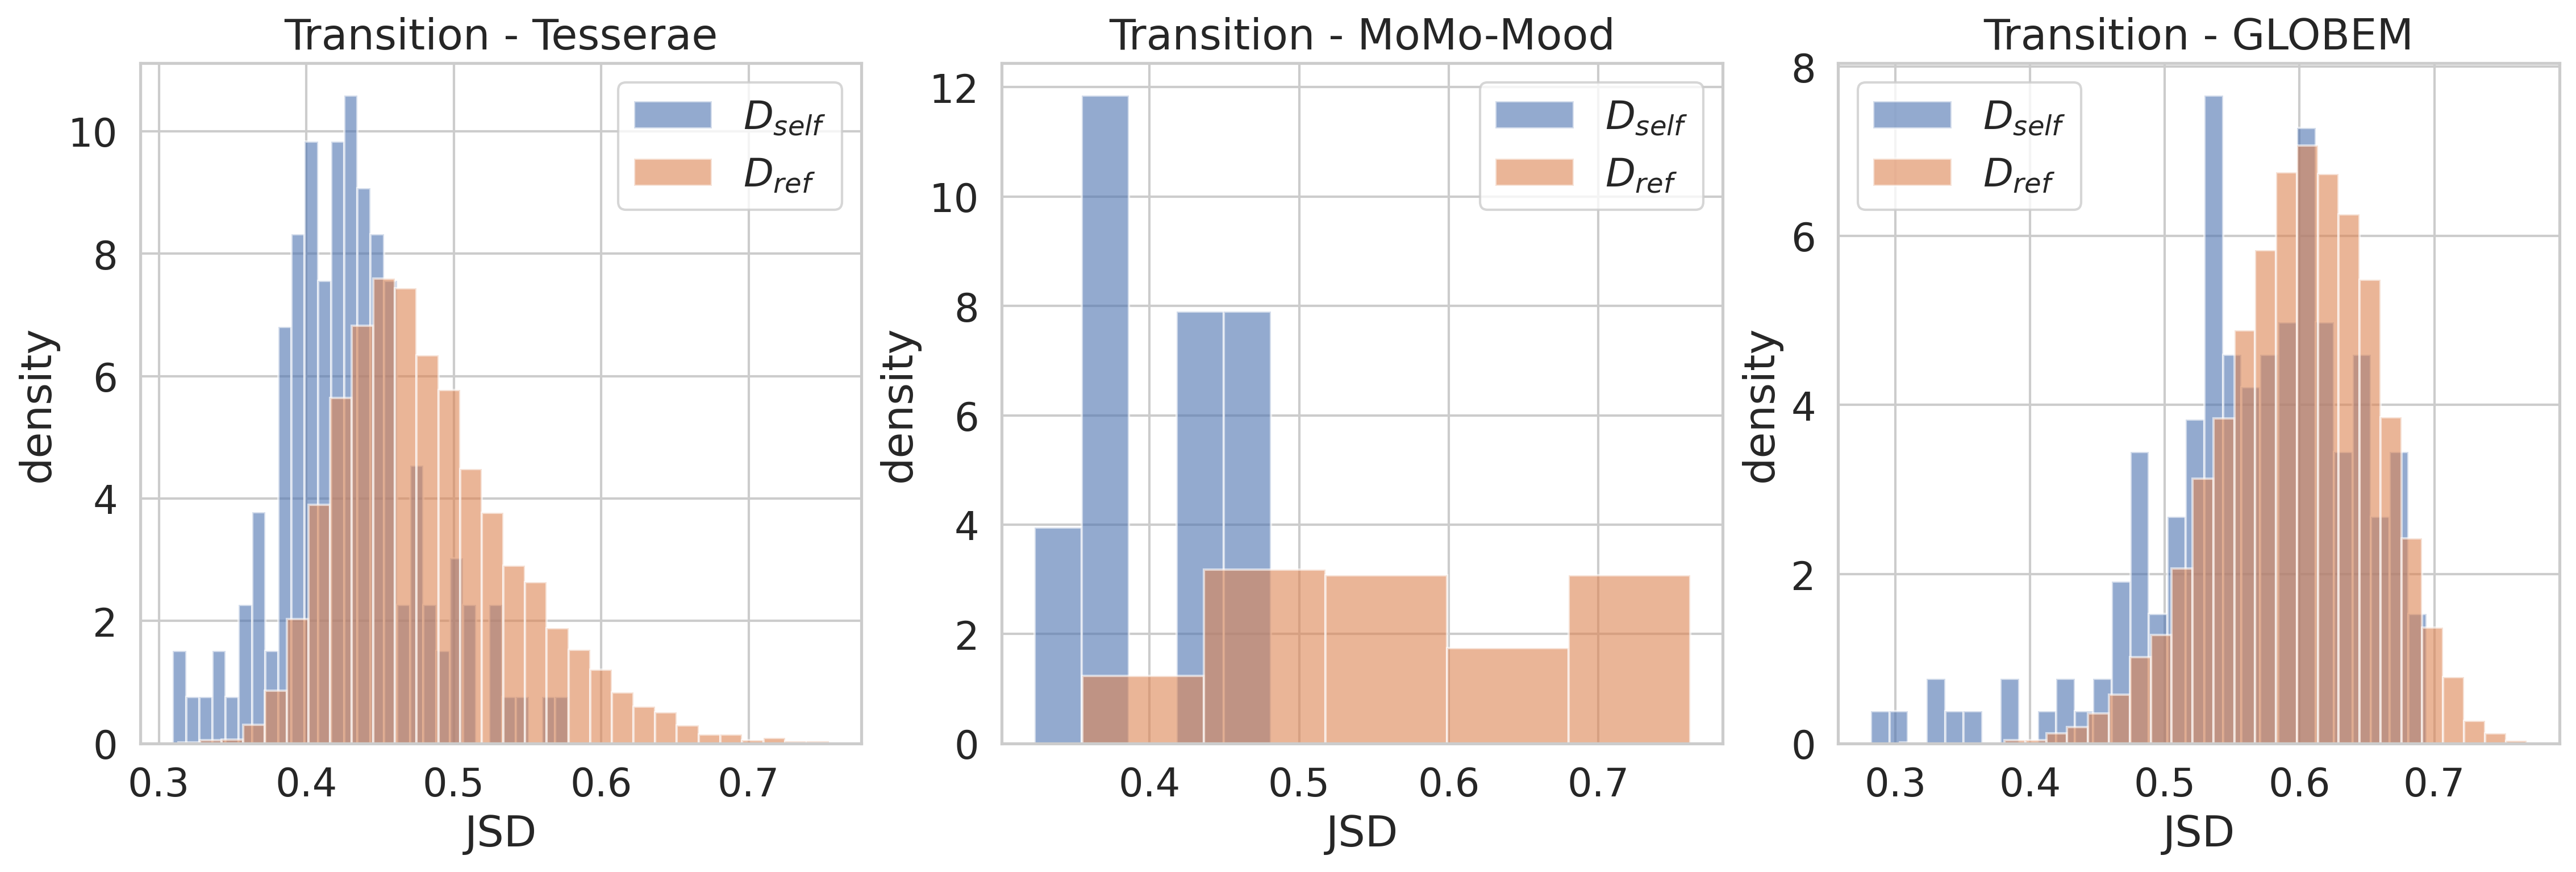
\includegraphics[width=1\linewidth]{figures/combined_transition_dself_dref_jsd.png}
    \caption{Transition signature}
    \label{fig:transition-signature}
\end{figure}

The within-person (\(d_{\text{self}}\)) and between-person (\(d_{\text{ref}}\)) distances of transition matrices for Tesserae and MoMo-Mood are shown in \autoref{fig:transition-signature}, generally depicting distribution with similar shape to the self and reference distance of routine signatures. In both studies, individual transition signatures persist across time segment and were also distinguishable from others. In Tesserae, this distance was \dself{0.481}{0.044}, smaller than the average reference distance \dref{0.537}{0.029} (\dselfdrefp{255.65}{-12.86}{0.0}). Similarly, in MoMo-Mood, we found \dself{0.458}{0.055} compared to \dref{0.600}{0.046}, \dselfdrefp{28.62}{-7.79}{0.0}.

Note that we did not perform this analysis on GLOBEM due to methodological difference in how cluster of routine was found. In GLOBEM, the clustering algorithm was applied on each wave independently, meaning that the latent routines from each wave may carry different meanings, making transition matrix non-comparable without an explicit label-alignment procedure.

\subsection*{Factors predicting persistence of routine signature}\label{sec3.3}

Prior work has linked sociodemographic factors \cite{luong2023impact, luong2024sleep, kulshrestha2021web} and personality traits \cite{centellegherPersonalityTraitsEgonetwork2017, alessandrettiUnderstandingInterplaySocial2018, amon2022flexibility} to the persistence of various types of routines.  Whether these relationships generalize to multifaceted routines remains unclear. We addressed this using two linear regression models: the first regressed routine-signature stability ($d_{\text{self}}$) on age, gender, and personality traits; the second used the same predictors to explain transition-signature stability ($d_{\text{self\_transition}}$). 

%Both models include study fixed effects with standard errors clustered by study to account for between-study differences.

\begin{table}[ht]
\centering
\small
\begin{tabular}{@{}lrrr rrr@{}}
\toprule
& \multicolumn{3}{c}{\textbf{$d_{self}$}} & \multicolumn{3}{c}{\textbf{$d_{self\_transition}$}} \\
\cmidrule(lr){2-4}\cmidrule(l){5-7}
& \textbf{$\beta$} & \textbf{SE} & \textbf{p-value} & \textbf{$\beta$} & \textbf{SE} & \textbf{p-value} \\
\midrule
\textbf{Fixed effects} \\
Age [25--34]      &  0.001 & 0.011 & 0.968 & -0.014 & 0.005 & 0.228 \\
Age [35--44]      &  0.011 & 0.012 & 0.458 & -0.030 & 0.006 & 0.134 \\
Age [45--54]      & -0.005 & 0.015 & 0.793 & -0.016 & 0.001 & \textbf{0.026}* \\
Age [55--64]      &  0.021 & 0.006 & 0.084\textsuperscript{.} & -0.011 & 0.004 & 0.203 \\
Gender (Male)     & -0.006 & 0.002 & 0.091\textsuperscript{.} &  0.002 & 0.003 & 0.616 \\
Openness          & -0.003 & 0.003 & 0.455 &  0.000 & 0.008 & 0.993 \\
Conscientiousness & -0.005 & 0.006 & 0.482 & -0.002 & 0.004 & 0.742 \\
Extroversion      & -0.004 & 0.001 & 0.073\textsuperscript{.} &  0.010 & 0.008 & 0.430 \\
Agreeableness     & -0.003 & 0.003 & 0.371 &  0.004 & 0.002 & 0.368 \\
Neuroticism       &  0.004 & 0.005 & 0.458 &  0.009 & 0.007 & 0.430 \\
\midrule
\textbf{Model info} \\

RMSE              & \multicolumn{3}{c}{0.08} & \multicolumn{3}{c}{0.04} \\
Adj.\ $R^2$       & \multicolumn{3}{c}{0.33} & \multicolumn{3}{c}{0.02} \\
\bottomrule

\end{tabular}
\caption[OLS of routine signatures]{OLS estimates for (i) signature persistence ($d_{\text{self}}$) and (ii) transition signature persistence ($d_{\text{self,transition}}$). All models include study as fixed effects; standard errors are clustered by study. Age is a categorical predictor with $<\!25$ as the reference. \textsuperscript{.}\,$p<.10$, *$p<.05$, **$p<.01$.}
\label{tab:ols_signature}
\end{table}


\autoref{tab:ols_signature} presents the OLS results. Overall, we find marginal associations between gender (female less regular than male, $\beta=-0.006$, $p=.091$) and extroversion (higher extroversion linked to lower routine stability, $\beta=-0.004$, $p=.073$) with routine persistence ($d_{\text{self}}$). For transition persistence ($d_{\text{self,transition}}$), no significant associations were found except for the 45--54 age group, which showed lower transition stability compared to the youngest group ($\beta=-0.016$, $p=.026$).

\section*{Discussions}\label{sec4}  

This work exemplified the persistence characteristics of human's routine observed in previous studies, as well as limitations of this persistence. We proposed a framework that models routines as latent behavioural classes and quantifies their persistence based on how individuals allocate their time across these classes. Across three independent studies, we find that individuals consistently devote similar proportions of time to their routines, forming distinctive routine signatures that remain stable over shorter monitoring periods. However, when examined over longer timescales—such as across years with substantial gaps between data collections—this persistence diminishes, suggesting that routine signatures are sensitive to large temporal separations. Although these signatures are individual-specific, they are not well explained by demographic or personality factors.

To contextualize our findings, we draw comparisons with prior work on the stability of human behavior. The social signature—the tendency for individuals to distribute their communication efforts unevenly across social contacts—has been shown to remain stable over time within small cohorts \cite{saramaki2014persistence}, and later generalized to larger and more diverse populations \cite{heydari2018multichannel, iniguezUniversalPatternsEgocentric2023}. Similar forms of temporal persistence have also been observed in other routine modalities, including mobility patterns \cite{alessandrettiUnderstandingInterplaySocial2018, alessandretti2020scales} and online behaviors \cite{kulshrestha2021web, malmi2016you}. Our work extends these findings by integrating multiple behavioral domains and representing daily life as a distribution over latent routine classes. We show that individuals not only allocate time unevenly across a limited number of dominant routines, but also maintain a distinctive pattern of transitions between them. This former structure is similar to that of social signatures: just as most communication time is concentrated on a few close ties, much of one’s daily life is organized around a small set of core routines, such as weekday-weekend. For the latter, we find similarity to the stability of human mobility patterns in both physical and digital spaces. Individuals tend to follow consistent and repeatable paths, such as commuting to and from the same locations, or navigating through sequences of websites or applications. Similarly, this pattern generalizes to daily routines more broadly: people transition between behavioral states in structured and habitual ways, thus forming individualized transition routines.

While prior work has demonstrated that social signatures remain stable over consecutive periods \cite{saramaki2014persistence}, we examined routine signatures in a more challenging context: shorter observation windows and larger temporal gaps between measurement periods. This experiment, conducted on the third study, resulted reduced stability in routine signatures, of which individual's signature was not distinguishable. This finding can be explained by several factors. First, the short observation window (50.6 days, compared to 90-day window in Tesserae and MoMo-Mood), may introduce challenges to capture the full variability of an individual's routine structure, thereby reducing the robustness of signature estimation. Second, the one-year gap between consecutive waves in GLOBEM likely introduced behavioral drift due to life changes or societal disruptions, such as the COVID-19 pandemic. Third, the GLOBEM cohort primarily consisted of university students, who typically share synchronized schedules (e.g., academic calendars, exams, and structured social life). This synchronization may in turn reduces the inter-individual variability and limit the distinctiveness of routine signatures.

Our study has several limitations, both in the data's properties and methodology. On the data side, although we considered multiple routine modalities, common routines like mobility and communication were not included due to missingness and sparsity of features. GPS signals showed substantial missingness across datasets, so we excluded mobility features to avoid biased estimates. Communication activity was logged only via calls and SMS; without app-based messaging, the communication feature space was sparse and zero-inflated. As a result, clustering on these variables tended to produce a dominant “no communication” cluster that mainly separated participants with any call/SMS activity from those with none. On the methodology side, our clustering approach are also limited in many ways. While the number of latent classes was selected via model selection, the model remains unsupervised in nature, meaning that the resulting clusters can vary between population or carry different meanings, and making interepratebly hard. Furthermore, by clustering via a bag-of-days method, we ignored the sequential temporal order of routines. Even so, we observed a clear weekday–weekend split among clusters, indicating strong periodicity that emerges even without explicit temporal modeling. Future work can consider temporal dependencies via appropriate methods such as Markov model \cite{liuIntraindividualPhenotypingDepression2024, leaningUncoveringSocialStateMoMo-Mood025}.

\section*{Methods}\label{sec:methods}  

\subsection*{Study description}\label{sec:methods:study_desc}  

We used datasets gathered from three studies. These datasets were selected based on (1) common use of smartphone-based sensing, (2) the diversity of study populations in terms of geography (Finland and USA), occupation (students and white-collar workers), and mental health status (healthy controls and patients with mental disorder), (3) the diversity the nature of study designs— two continuous monitoring studies and one spanning multiple years. These features aid the generalizability of the findings and .. help test the validity of routine signature. An overview of feature processing and bulding of routine signature is presented in \autoref{fig:routine-sig-workflow}.

\textbf{Tesserae.} The Tesserae study recruited 757 information workers across the United States \cite{mattingly2019tesserae}. Participants were provided a Garmin Vivosmart 3 wristband to monitor physical activity, heart rate, sleep, and calories. Additionally, participants installed a custom smartphone app that passively tracked screen activity, data usage, charging behavior, location, and other phone states.

\textbf{MoMo-Mood.} The MoMo-Mood study involved patients diagnosed with major depressive episodes, including Major Depressive Disorder (MDD), Bipolar Disorder (BD), and Borderline Personality Disorder (BPD), as well as healthy controls (HC). The study recruited a total of 164 participants from Finland; 133 patients and 31 HCs \cite{aledavood2025multimodal}. Data were collected over a one-year period from smartphones using the AWARE platform \cite{ferreiraAWAREMobileContext2015}, which tracked screen activity, calls and SMS, charging behavior, location, and accelerometer.

\textbf{GLOBEM.} The GLOBEM study procured a multi-year passive sensing datasets of over 700 user-years of data from 497 unique college students \cite{xu2022globem}. Longitudinal data, including location, phone usage, calls, Bluetooth, physical activity, and sleep behavior, were collected from a mobile app and fitness trackers. The study spanned four years, with data collection occurring over a 10-week period each year, primarily during the spring semester. 

\subsection*{Features extraction and Preprocessing} \label{sec:methods:features_extraction}  

\textbf{Sleep.} Bed time, wake time, and sleep duration were collected directly from Garmin (Tesserae) and Fitbit (GLOBEM) fitness trackers. In MoMo-Mood, due to the lack of wearable devices, sleep was estimated using phone lock/unlock status, with the longest lock episode considered sleep. To assess the validity of this proxy, sleep parameters from the same participants were compared to those derived from actigraphy during a two-week validation phase . The comparison revealed a slight bias but demonstrated adequate correlation between the two methods.

\textbf{Physical activity.} This routine was measured using step count data collected from fitness trackers in the Tesserae and GLOBEM studies. In contrast, for Tesserae, where no fitness trackers were used, mobility was estimated using the standard deviation of the accelerometer magnitude \cite{ravi2005activity}. Accelerometer readings displayed a clear 24-hour rhythm, consisted of higher activity levels during the day, a peak around a specific hour, and a gradual decline toward the end of the day, reflecting typical daily activity patterns. To capture daily patterns, activities were aggregated into four 6-hour time bins - proxy for four parts of the day (night, morning, afternoon, evening) - to construct a mobility rhythm. A daily average value was also computed.

\textbf{Device usage.} The hourly duration of screen use episodes was extracted. Daily rhythms for screen usage were constructed by aggregating the hourly measures into 4-hour bins. 

\textbf{Demographics and personality traits.} Baseline demographics (age, gender, occupation) were recorded at enrollment. In Tesserae, age was available only in aggregated bins; to ensure comparability, we applied the same binning across all studies: $<!25$, 25–34, 35–44, 45–54, and 55–64. Personality traits were assessed with the BFI-10 \cite{rammstedt2007measuring} in Tesserae and GLOBEM and the NEO-60 \cite{costa1992neo} in MoMo-Mood. Because Tesserae reported personality traits as aggregate scores on a 1–5 scale, we linearly rescaled the MoMo-Mood and GLOBEM trait scores to the same $[1,5]$ range for cross-study comparability.

\textbf{Exclusion and normalization}: The records from the first and last day of any user were excluded due to high likelihood of data incompleteness. We excluded participants with fewer than 14 days of data for clustering task. Any day with missing data on device usage, physical activity, or sleep were excluded. Each feature was z-normalized within participants, allowing the model to focus on intra-individual variability. The resulting daily vector contained 13 features (see \autoref{tab:features_list}). Dimensionality reduction was not performed because (1) the feature space is reasonably small and (2) retaining the original variables preserves interpretability of the subsequent clustering results.

\begin{table}[ht]
    \centering
    \begin{tabular}{ll}
        \toprule
        \textbf{Routine} & \textbf{Features} \\
        \midrule
        Physical activity & Step count (MoMo-Mood, GLOBEM); accelerometer (Tesserae): daily average + MAEN \\
        Sleep             & bedtime, wake time, sleep duration \\
        Device usage      & Screen usage duration: daily average + MAEN \\
        \bottomrule
    \end{tabular}
    \caption{List of daily behavioral features, grouped by routine domain. MAEN = Morning, Afternoon, Evening, Night segments.}
    \label{tab:features_list}
\end{table}

\subsection*{Building routine cluster using GMM}\label{sec:methods:building_cluster}

For each participant, we formed an $M \times N$ matrix of daily features ($N$ features over $M$ days) and fit a $K$-component Gaussian Mixture Model (GMM). The $K$ multivariate Gaussian components (means $\boldsymbol{\mu}_k$, covariances $\boldsymbol{\Sigma}_k$, weights $\pi_k$) represent latent routines. This approach captures both the mean behavioral profile (via the components' mean) and the variability and correlation among features (via the covariance matrices).
Compared to clustering methods like K-Means, GMM offers greater flexibility. First, GMM supports soft clustering, meaning each day is assigned to multiple routine types with varying probabilities, modelling the transition nature of human behavior. Second, each GMM component can be parameterized by the full covariance structure, which captures the interdependencies between routines. For instance, increased phone activity late at night may correlate with delayed bedtime. Third, probabilistic assignments of cluster enable detection of anomalous routines, i.e. days which do not fit into any type of routines.

GMM has two main hyper-parameters: the number of components \(k\) and the covariance type (full, tied, diagonal, or spherical). 
Model selection was based on the Bayesian Information Criterion (BIC), with lower values indicating better fit. For model with full covariance matrix, we quantified cluster separation by computing all pair-wise Bhattacharyya distances. 
For two multivariate Gaussian clusters \(p_1 \sim \mathcal{N}(\boldsymbol{\mu}_1, \boldsymbol{\Sigma}_1)\) and \(p_2 \sim \mathcal{N}(\boldsymbol{\mu}_2, \boldsymbol{\Sigma}_2)\), the Bhattacharyya distance is

\[
D_B(p_1,p_2)
    = \frac{1}{8}\,
      (\boldsymbol{\mu}_1 - \boldsymbol{\mu}_2)^{\mathsf T}
      \boldsymbol{\Sigma}^{-1}
      (\boldsymbol{\mu}_1 - \boldsymbol{\mu}_2)
      + \frac{1}{2}\,
        \ln\!\left(
          \frac{\det\boldsymbol{\Sigma}}
               {\sqrt{\det\boldsymbol{\Sigma}_1\,\det\boldsymbol{\Sigma}_2}}
        \right),
\]

where
\[
\boldsymbol{\Sigma} = \frac{1}{2} \left( \boldsymbol{\Sigma}_1 + \boldsymbol{\Sigma}_2 \right)
\]
is the average covariance matrix, and \(\boldsymbol{\mu}_1,\boldsymbol{\mu}_2\) are the cluster mean vectors. Larger values indicate better separation between clusters.

We assigned each day to one of the resulting components. This clustering process was carried out independently for each study. For GLOBEM, the dataset spanned multiple academic years, so we fitted the clustering model separately for each year (semester). The tuning process is detailed in Appendix 1.

\subsection*{Routine signature}\label{sec:methods:signature}  

Social signature describes how individuals persistently distribute their communication efforts across their social contacts \cite{saramaki2014persistence}. We extended this concept by introducing the notion of a routine signature—the characteristic way in which individuals distribute their time across recurring patterns of daily behavior. Our concept aims to capture the persistence in the way individuals structure their daily lives across different types of routines.

For each participant, we represented every day in terms of behavioral features and assigned GMM cluster. Then, we summarized how often each cluster occurred for that participant by counting the number of days assigned to each cluster. To obtain a comparable distribution across individuals, these counts were normalized into proportions, giving the fraction of the participant’s days that belonged to each cluster.  

The clusters were then ranked in descending order of frequency (rank 1 = the most common cluster for that participant). 
The resulting vector of ranked proportions constitutes the \textit{routine signature} of that individual:

\begin{equation}
    \sigma_i = \left(
    \frac{n_{i1}}{\sum_j n_{ij}},\;
    \frac{n_{i2}}{\sum_j n_{ij}},\;
    \ldots,\;
    \frac{n_{ik_i}}{\sum_j n_{ij}}
    \right),
\end{equation}

where \(n_{ij}\) is the number of days participant \(i\) spent in cluster \(j\), and the elements are ordered so that \(\sigma_{i1} \geq \sigma_{i2} \geq \dots\).  

Intuitively, the routine signature reflects the individual pattern of time allocation across latent routines, independent of the cluster labels themselves. In line with the concept of social signatures, we expect this pattern to persist over time.

\begin{figure}[!htbp]
    \centering
    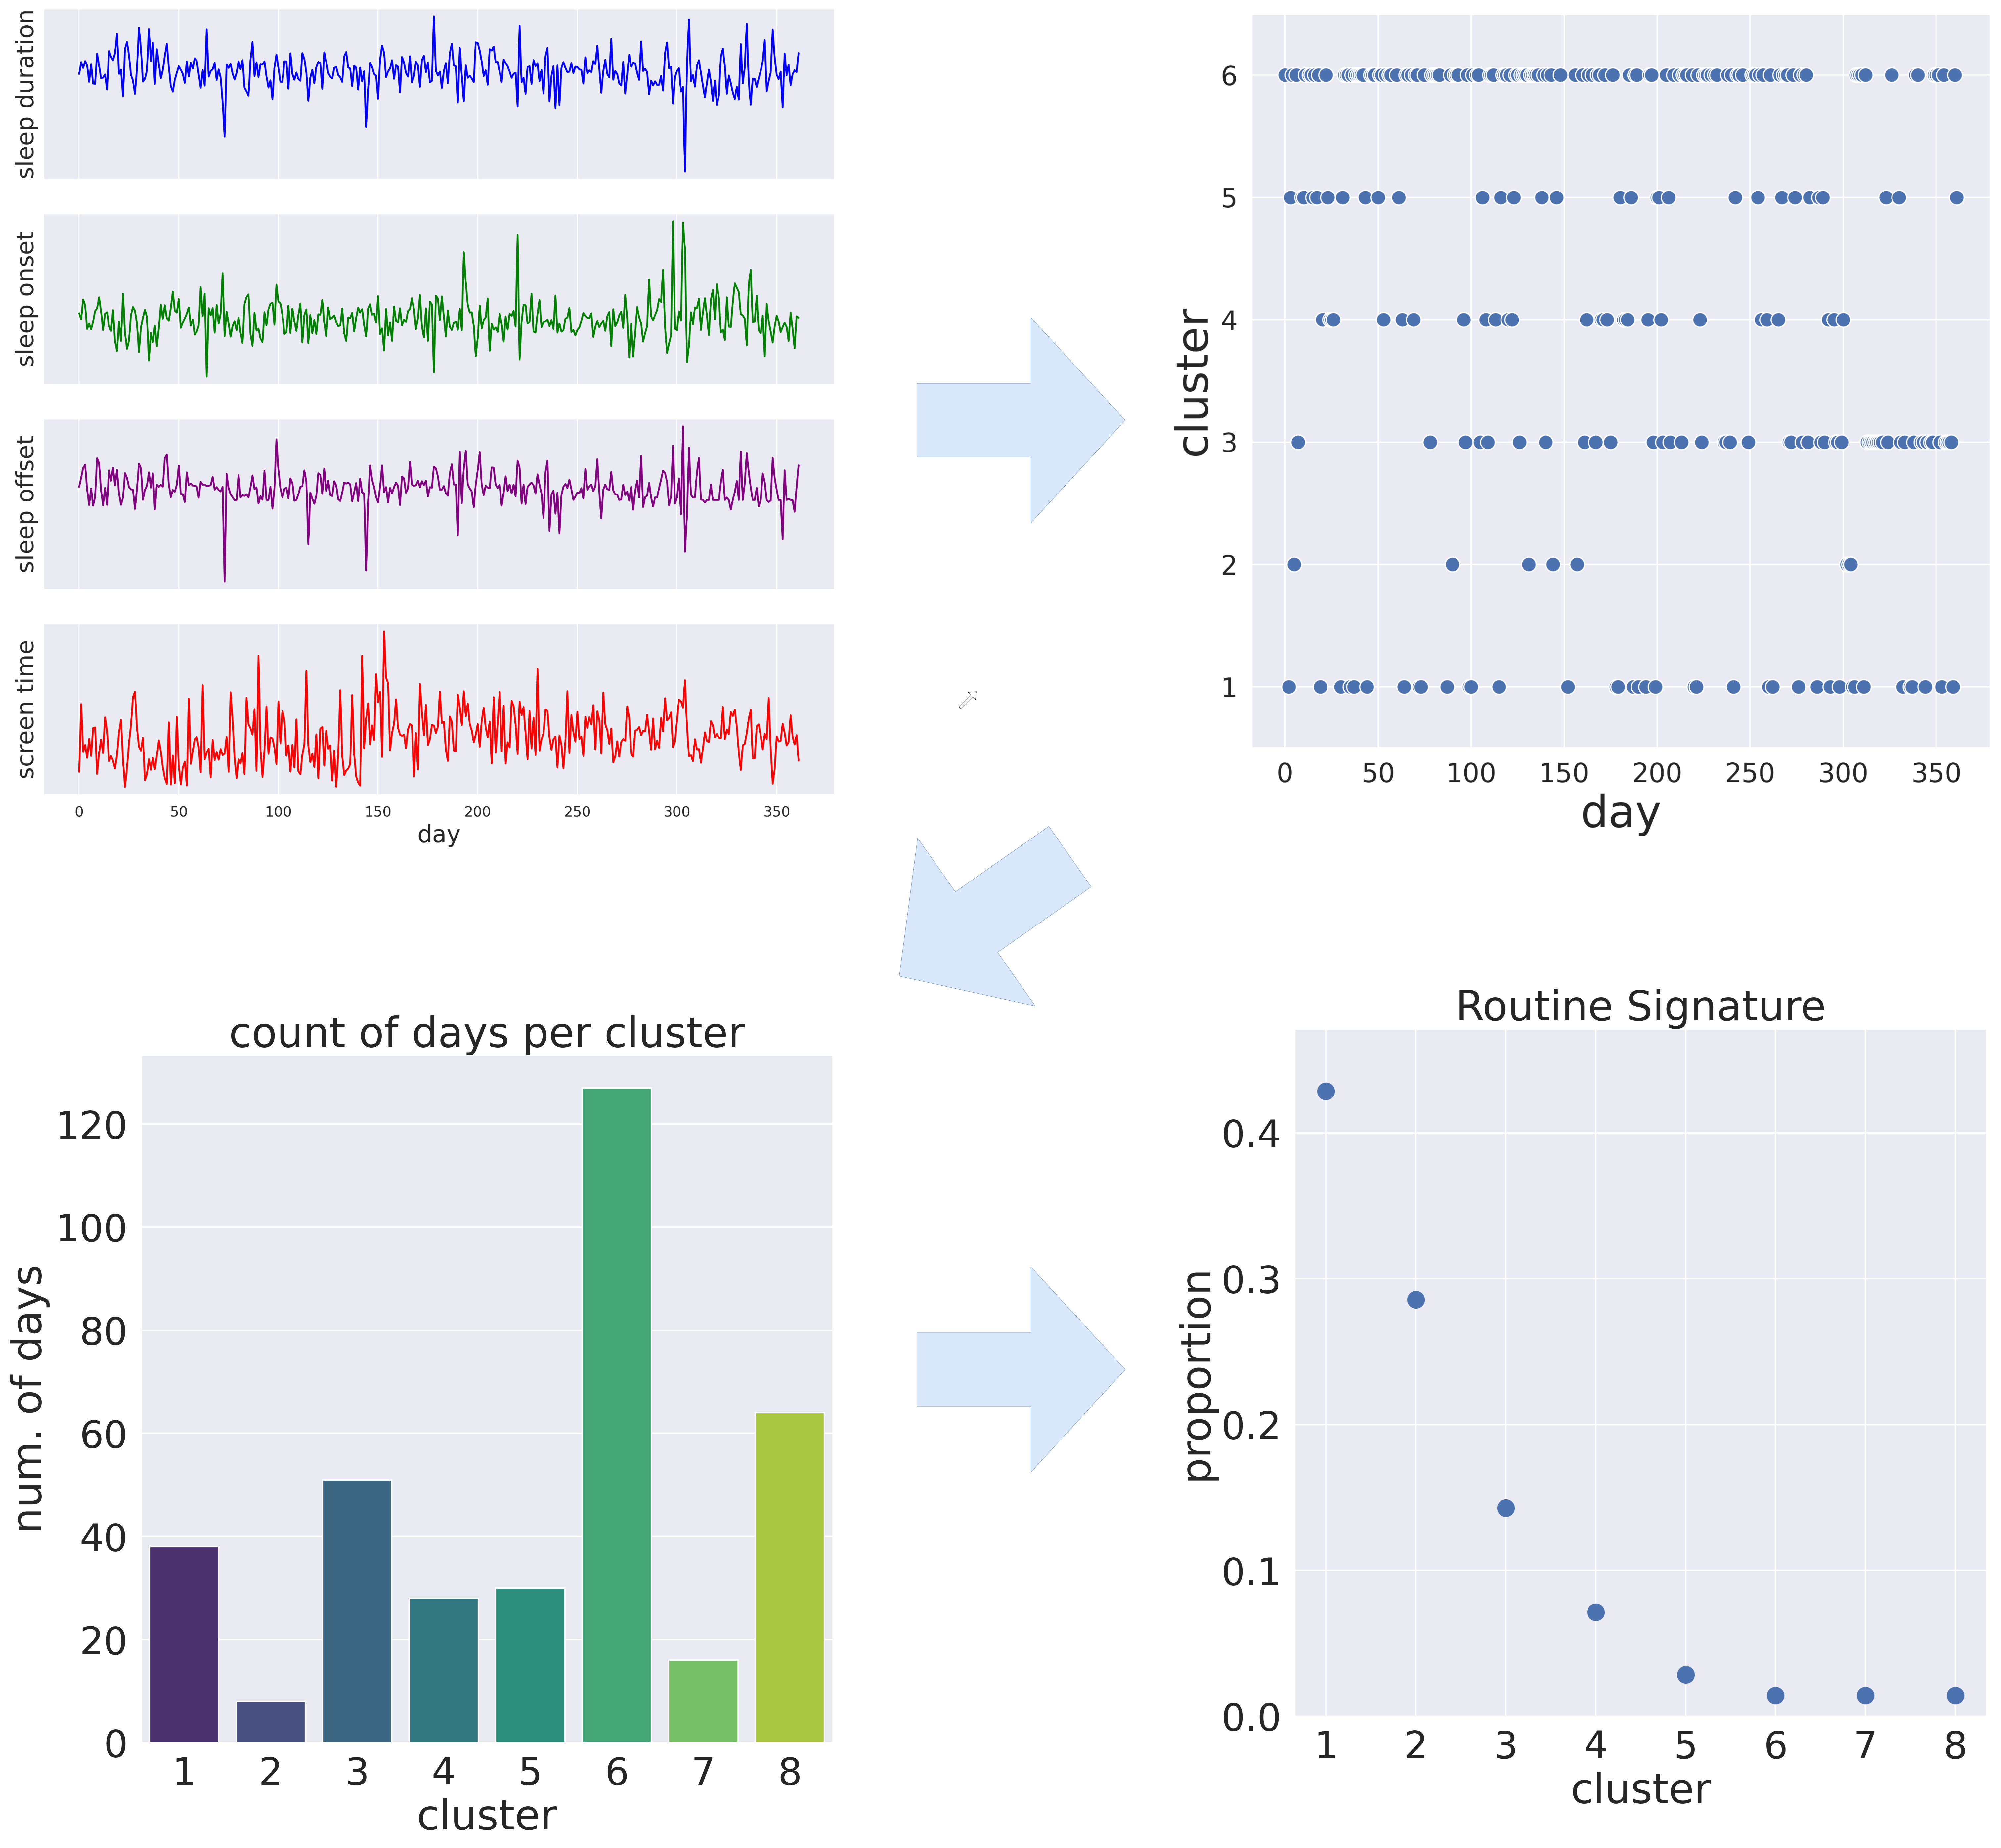
\includegraphics[width=\textwidth]{figures/digi-schema.png}
    \caption{Schematic description of routine signature. (A) Raw data capturing each person-day’s routine (e.g., sleep times, screen use, activity levels).
(B) Gaussian Mixture Model (GMM) fitted on the pooled person-day assigns each day to one of the routine clusters.
(C) For each individual, the number of days falling into each GMM‐defined cluster is computed and clusters are ranked by descending day‐counts.
(D) These counts are converted into proportions, giving each person’s routine signature.}
    \label{fig:routine-sig-workflow}
\end{figure}

\subsection*{Persistence of routine signatures}\label{sec:methods:signature_persistence}  

To quantify the persistence of routine signature, we examine how robust a person maintain the time allocated to their routine over time. For each person, the data was divided into 3 equal time segments. Due to the difference fin study design, the segmenting strategy was done differently for each dataset. For Tesserae and MoMo-Mood, each segment consisted of 90 days of data, hence we retained users with at least 270 data days. For GLOBEM, each segment equals to each wave, i.e 10 weeks of data, and we retained the users that participated in at least 2 waves of the study. The persistence of routine was defined as the distance between the routine signatures in consecutive time segments, using the Jensen-Shannon divergence (JSD) \cite{lin1991divergence}:

\begin{equation}
JSD(\sigma_1, \sigma_2) = H(\frac{\sigma_1 + \sigma_2}{2}) - \frac{1}{2}[H(\sigma_1) + H(\sigma_2)]
\end{equation}

where $\sigma_1$ and $\sigma_1$ are the social signatures defined in Eq. 1, and $H(\sigma)$ is the Shannon entropy of $\sigma$.

To determine how well one maintains their routines over time, we define $d_{self} =  d_{12}$. We validate individual's persistence against the population, by computing the reference distance $d_{ref} = \frac{1}{2}* (d_{i1j1} + d_{i2j2} )$. That is, we compute the routine signature in each time split of individual $i$ against that from the same time split of individual $j$.


% Uncomment to include appendix
%% Preamble additions (recommended)
% \usepackage{graphicx}
% \usepackage{subcaption}
% \usepackage{placeins}   % for \FloatBarrier
% \usepackage{float}      % if you want [H] placement (optional)

\section{Appendices}

\begin{appendices}

% ---------- A: GMM model tuning ----------
\clearpage                    % start this appendix section on a new page
\section{GMM model tuning}

Model tuning across all cohorts favored Gaussian mixtures with full covariance matrices, yielding lower Bayesian Information Criterion (BIC; lower is better) and higher average Bhattacharyya distances between components (greater separation). Performance improved up to \(K=8\) and then showed diminishing returns, so we fixed \(K=8\) for the main analyses. All principal findings were confirmed in a sensitivity analysis with \(K \in \{6,\ldots,11\}\).


\begin{figure}[p]
  \centering
  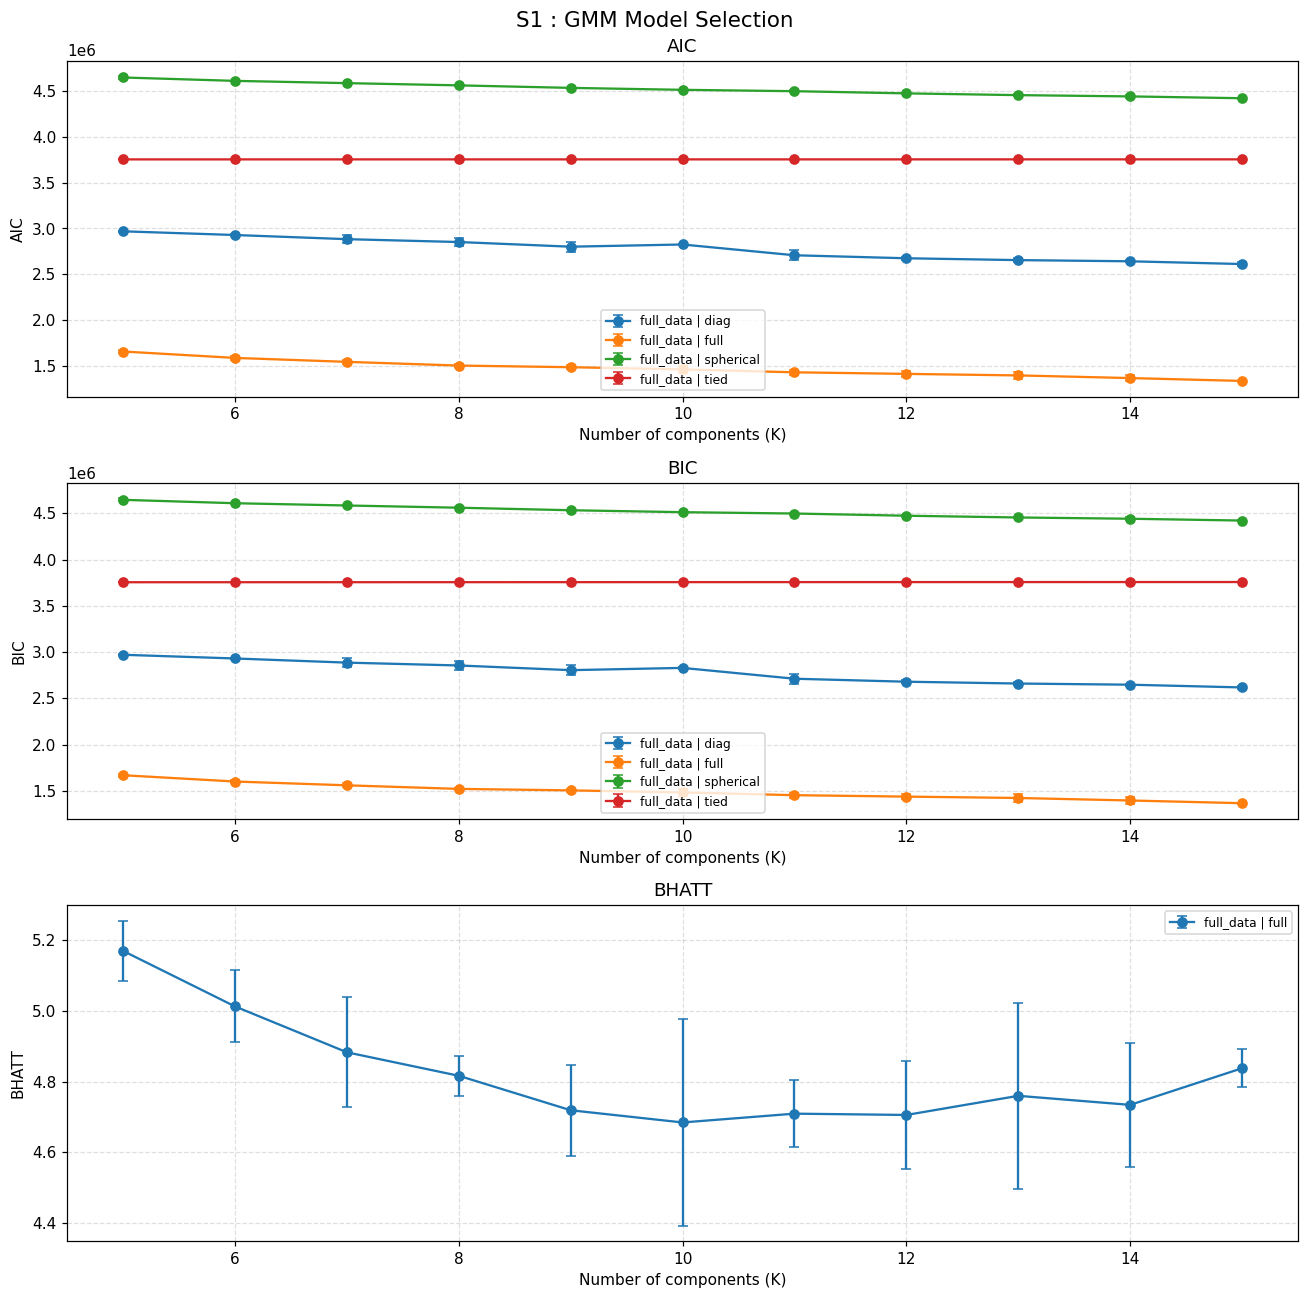
\includegraphics[width=\linewidth]{figures/appendix/tesserae_gmm_model_selection.png}
  \caption{Tesserae: Model selection}
  \label{fig:tesserae_model_selection}
\end{figure}

\begin{figure}[p]
  \centering
  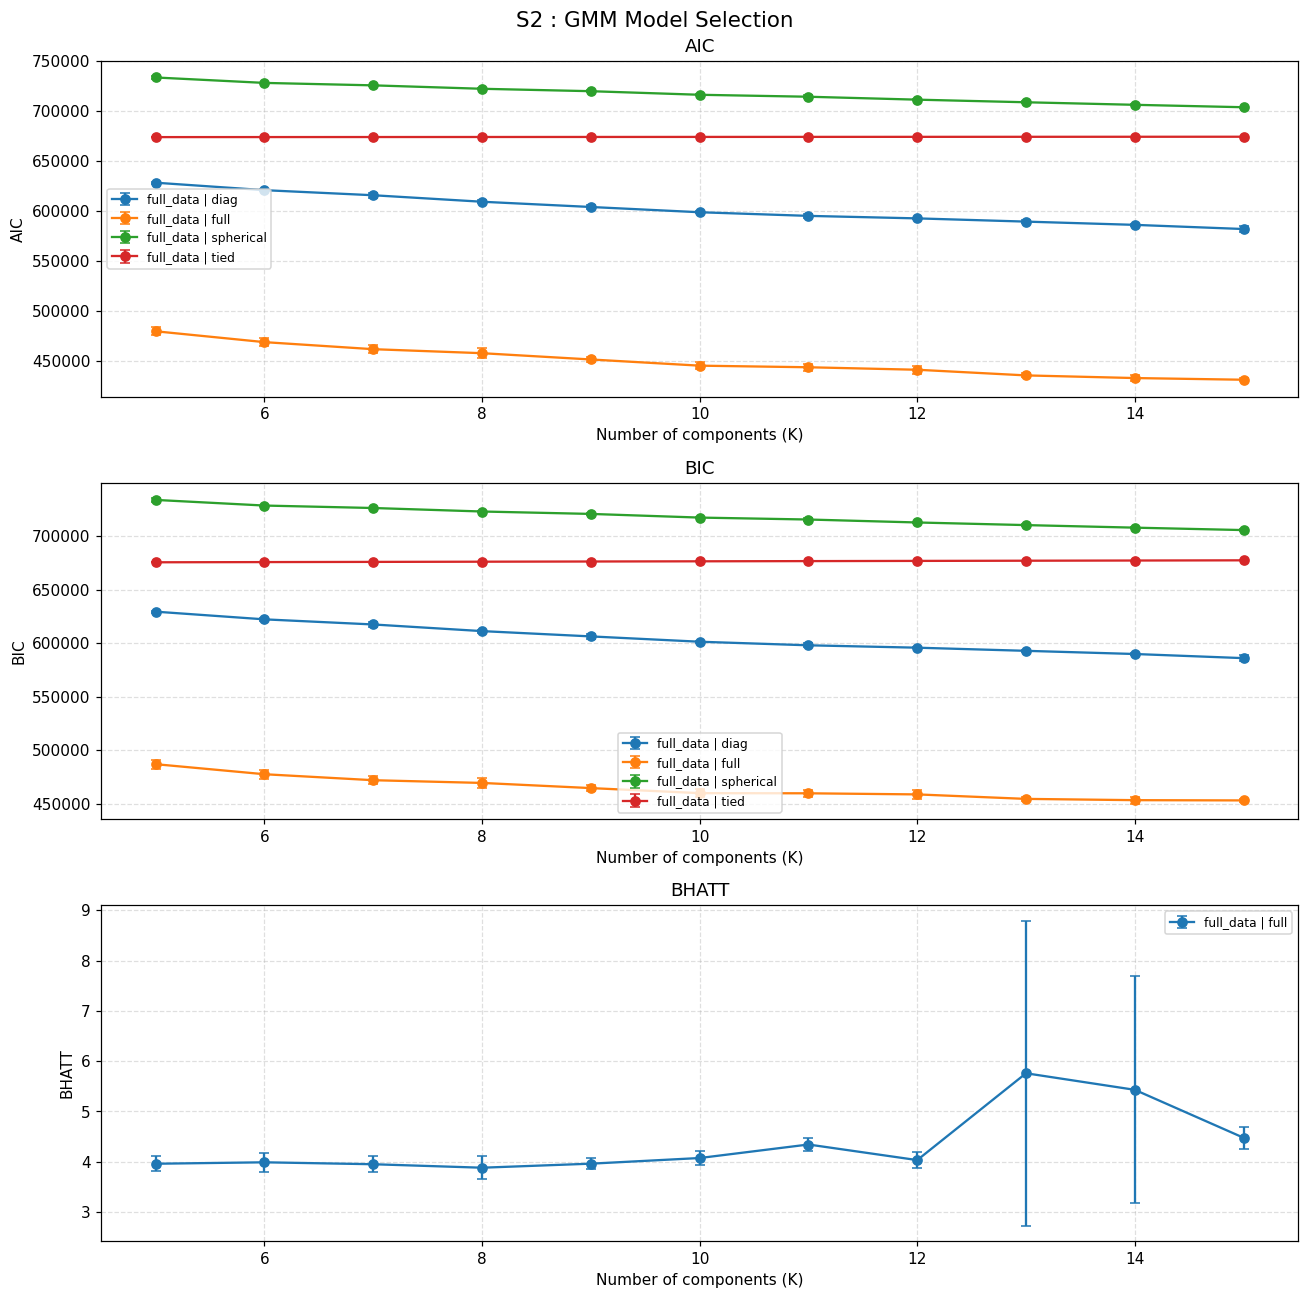
\includegraphics[width=\linewidth]{figures/appendix/momo_gmm_model_selection.png}
  \caption{MoMo-Mood: Model selection}
  \label{fig:momo_gmm_model_selection}
\end{figure}

\begin{figure}[p]
  \centering
  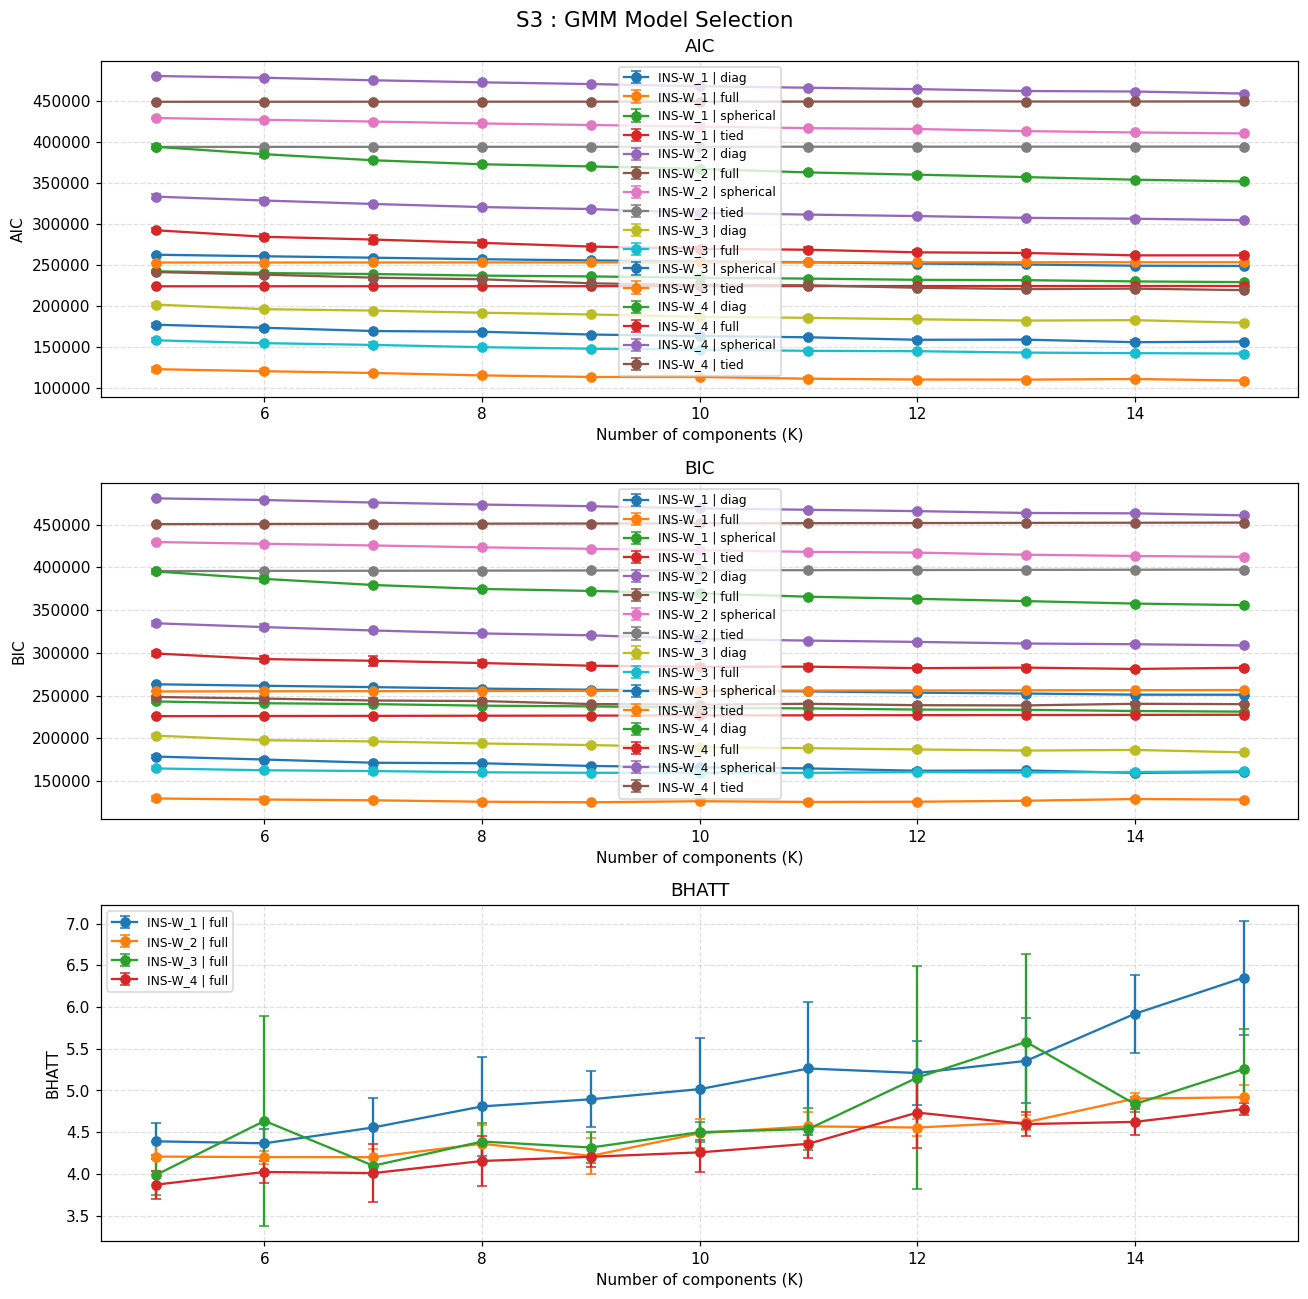
\includegraphics[width=\linewidth]{figures/appendix/globem_gmm_model_selection.png}
  \caption{GLOBEM: Model selection}
  \label{fig:globem_gmm_model_selection}
\end{figure}

\FloatBarrier                 % ensure these floats don’t spill into the next section

% ---------- B: Cluster properties ----------
\clearpage
\section{Cluster properties of MoMo-Mood and GLOBEM}

\autoref{fig:momo_centroid_summary} and \autoref{fig:globem_centroids} describe the cluster characteristics of the MoMo-Mood and GLOBEM studies, respectively. Across both datasets, a few dominant clusters account for the majority of time, while other clusters reflect free day routines, for example, elevated nightly activity or increased nighttime screen use.

\begin{figure}[p]
  \centering
  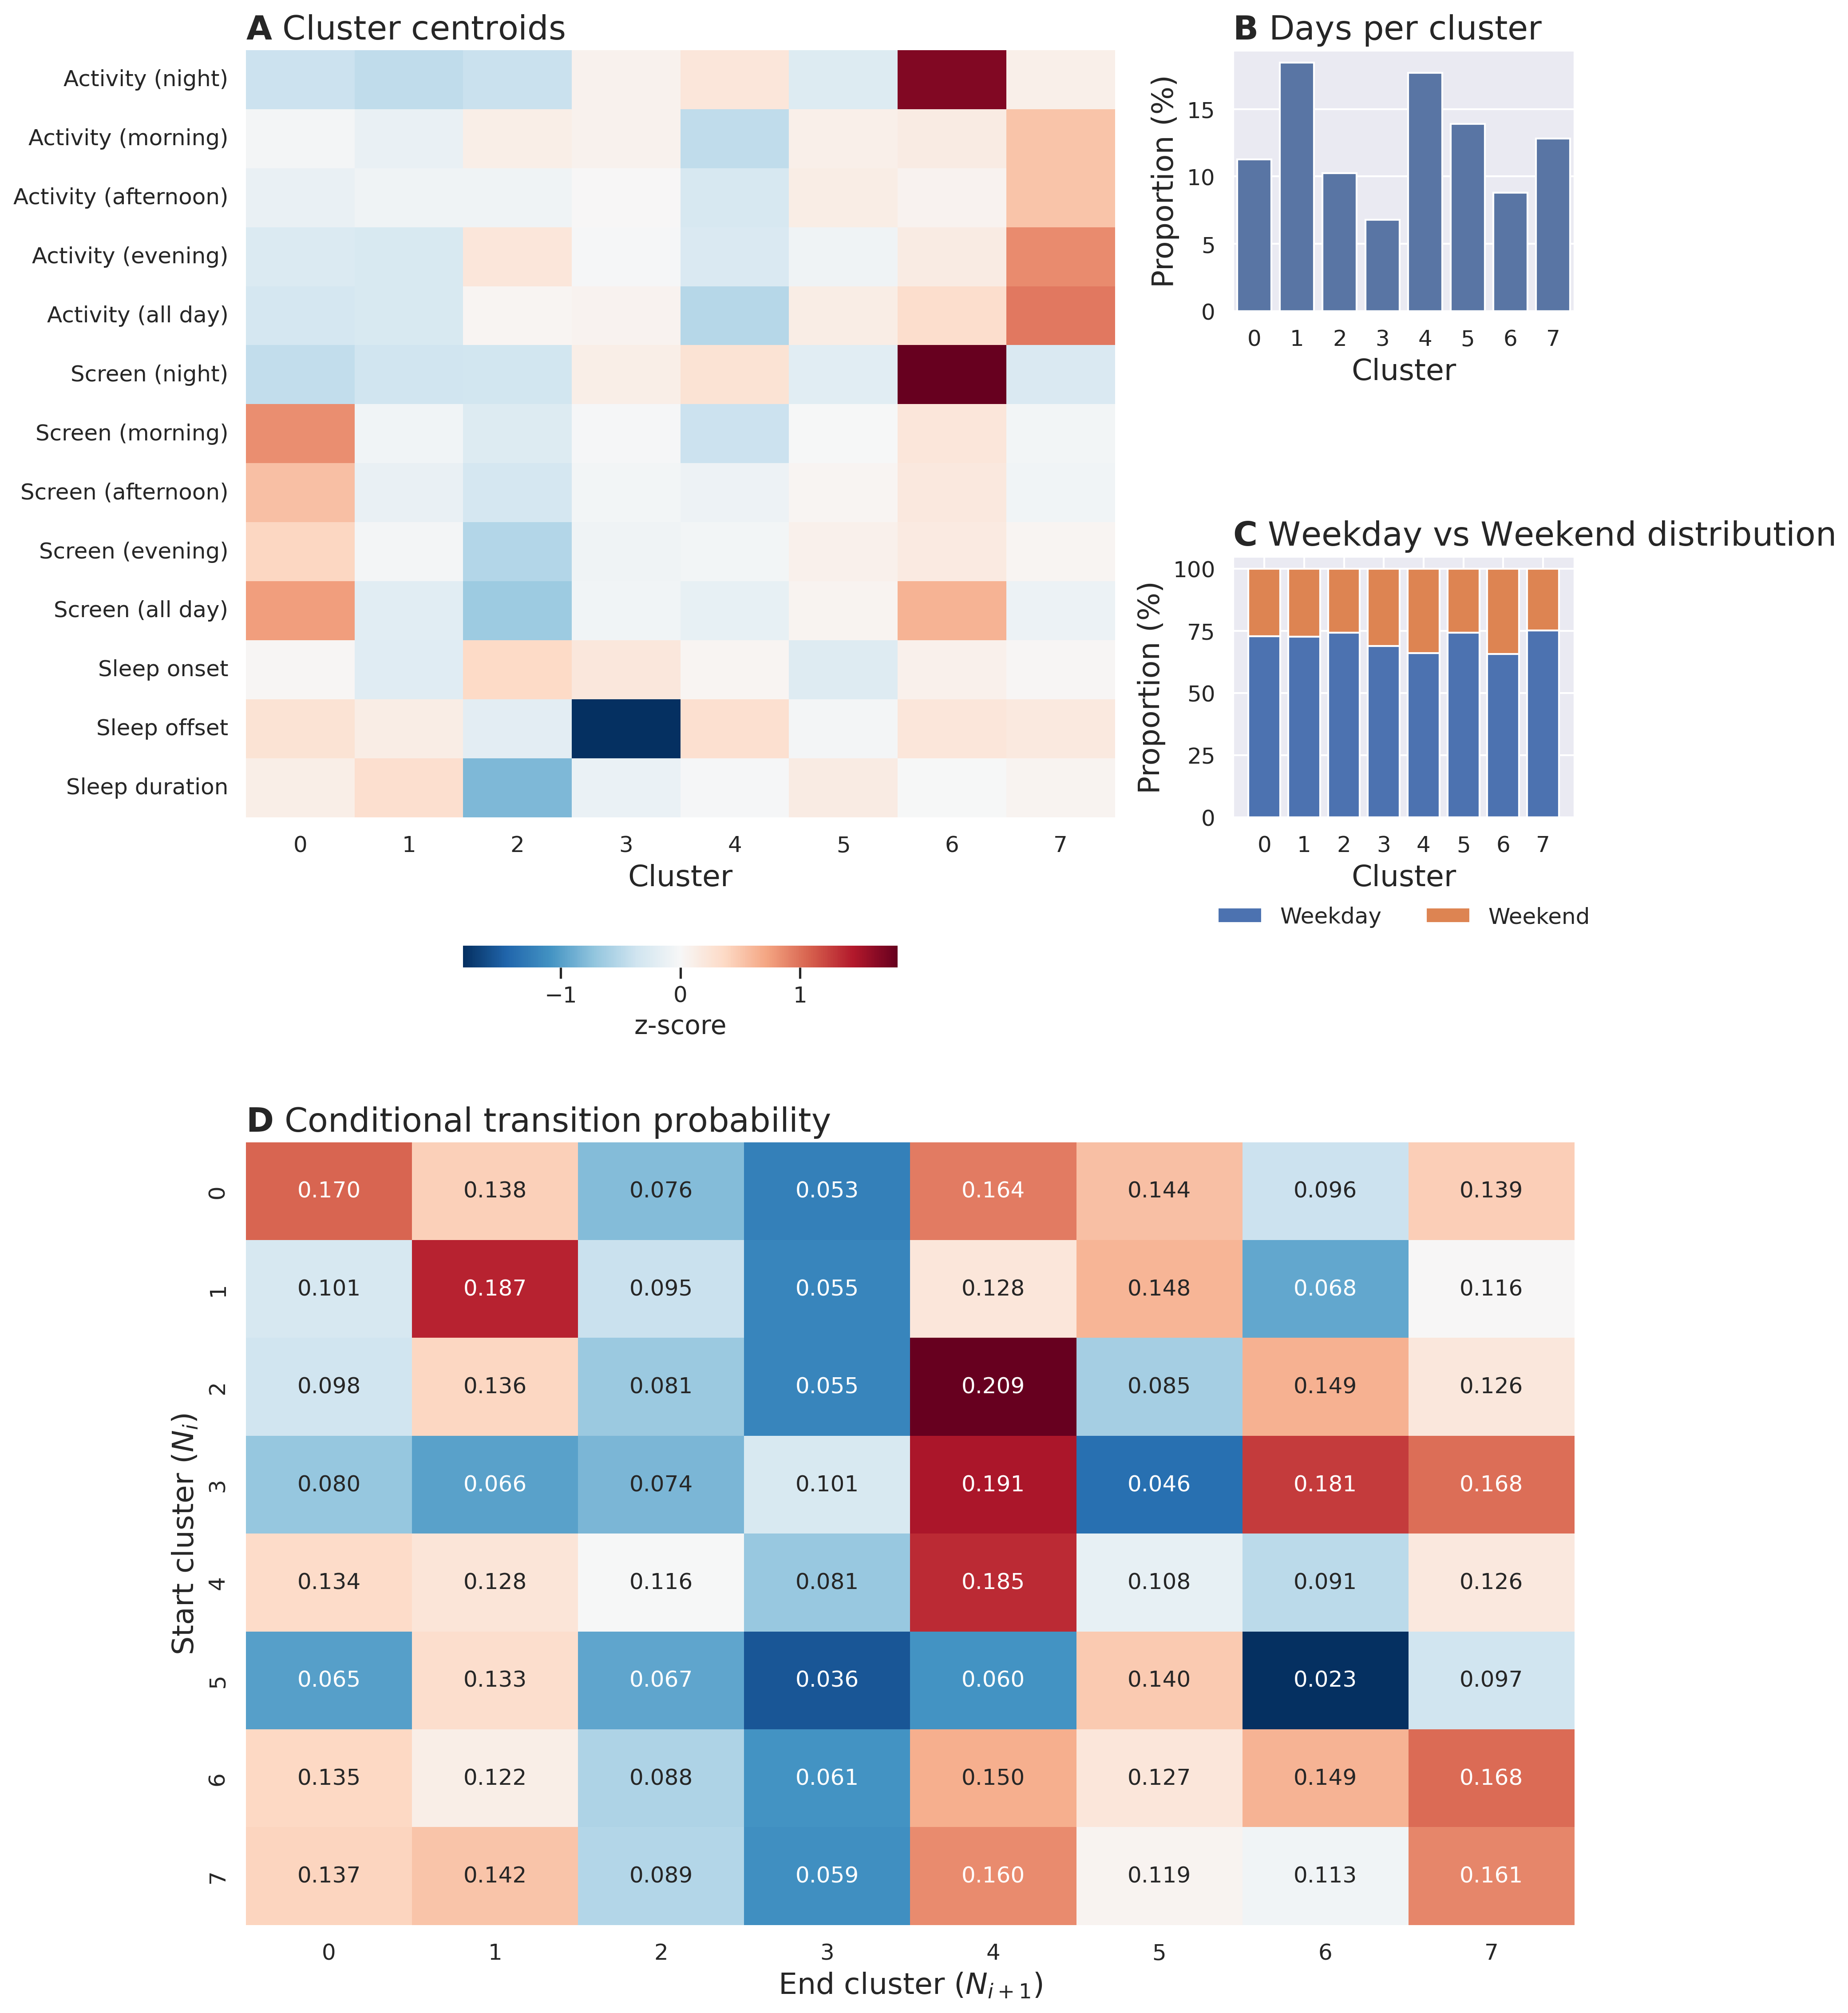
\includegraphics[width=\linewidth]{figures/appendix/momo_summary.png}
  \caption{MoMo-Mood: Cluster centroid characteristics}
  \label{fig:momo_centroid_summary}
\end{figure}

% 2x2 subfigures for GLOBEM centroid characteristics (example filenames 1–4)
\begin{figure}[p]
  \centering

  \begin{subfigure}[t]{0.485\textwidth}
    \centering
    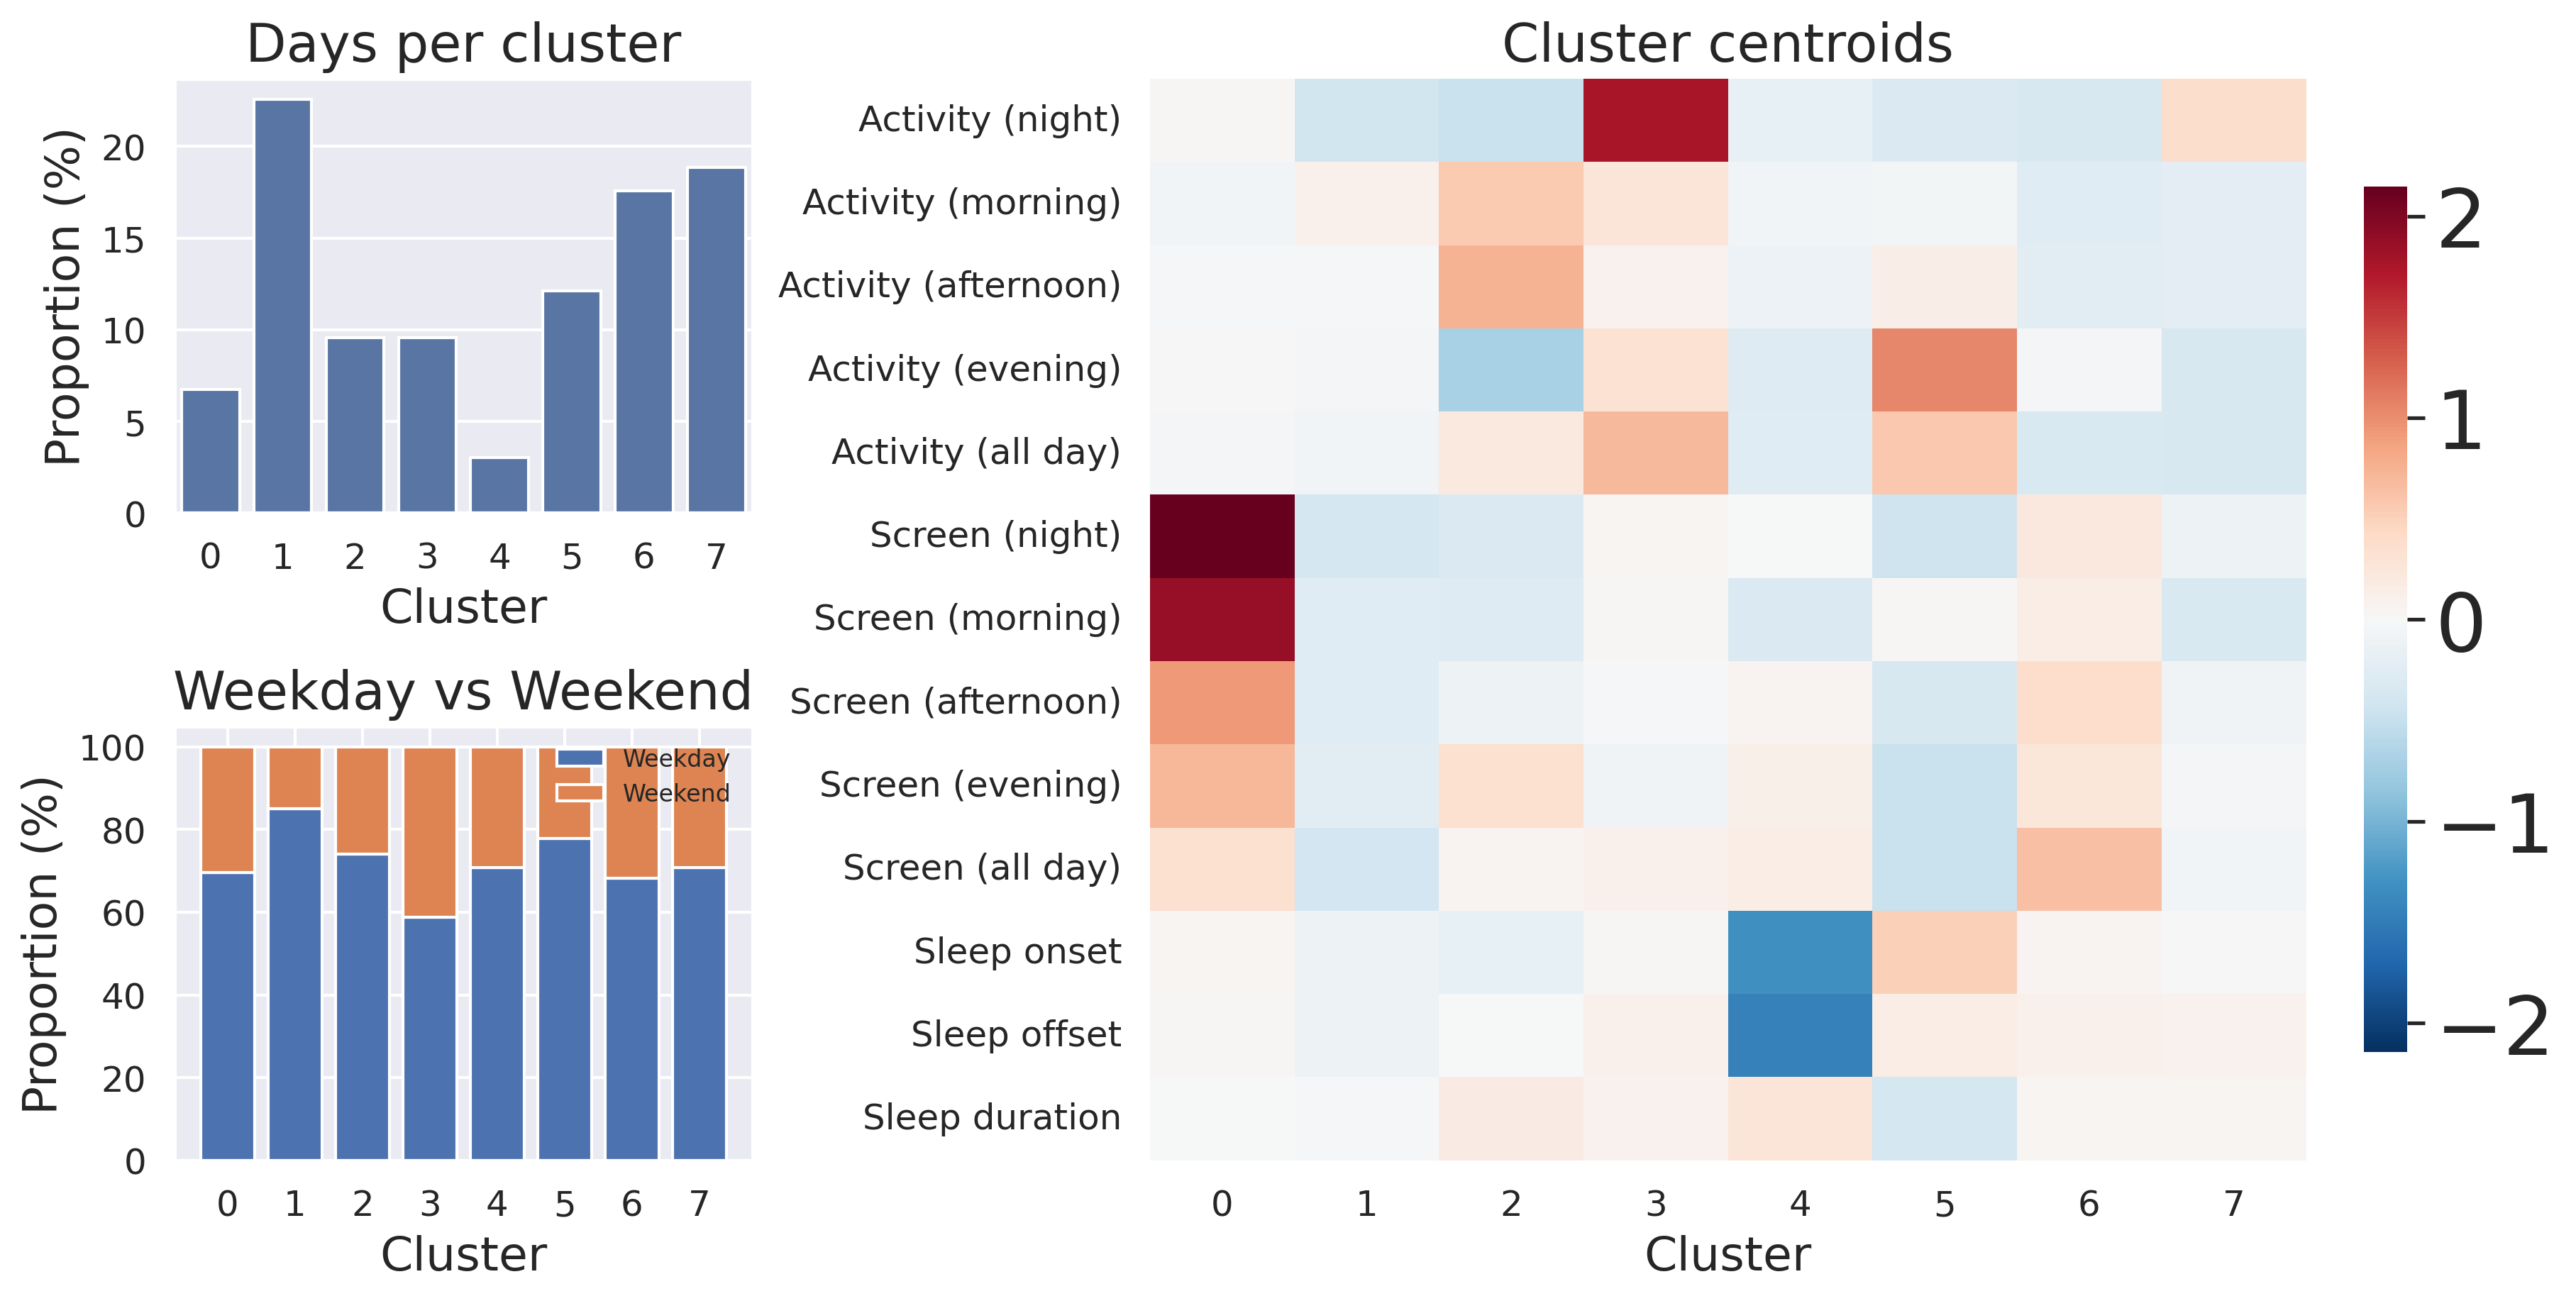
\includegraphics[width=\linewidth]{figures/appendix/globem_INS-W_1_summary.png}
    \caption{Cluster 1}
    \label{fig:globem_centroids_a}
  \end{subfigure}\hfill
  \begin{subfigure}[t]{0.485\textwidth}
    \centering
    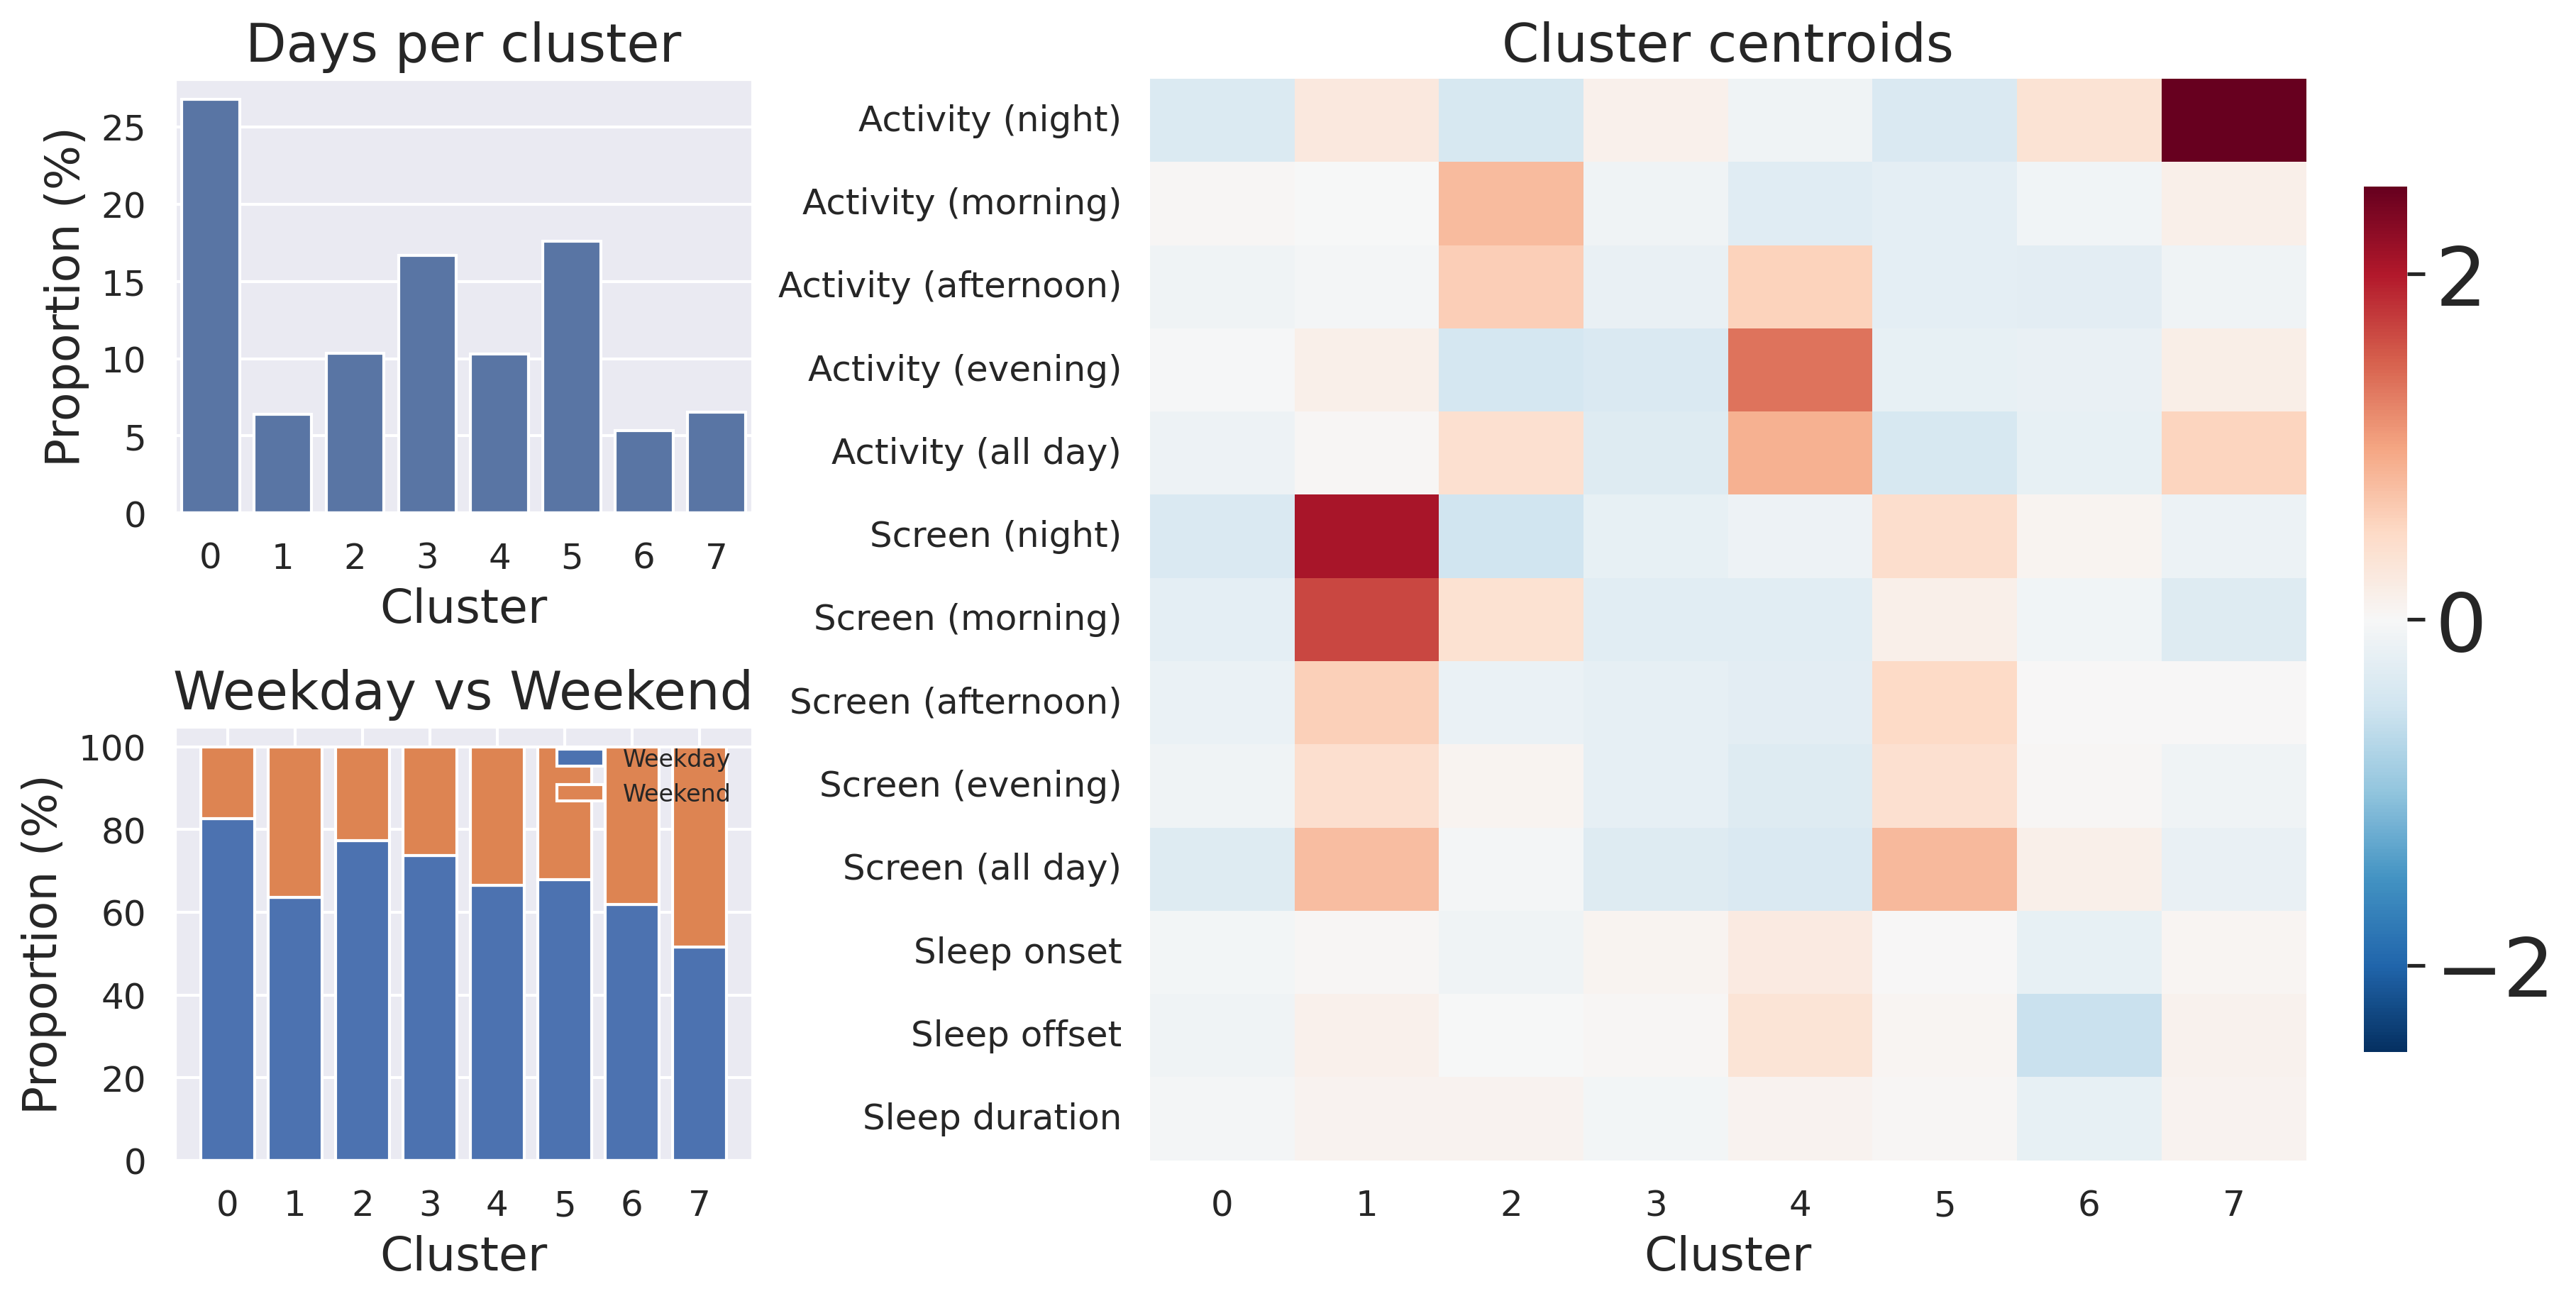
\includegraphics[width=\linewidth]{figures/appendix/globem_INS-W_2_summary.png}
    \caption{Cluster 2}
    \label{fig:globem_centroids_b}
  \end{subfigure}

  \medskip

  \begin{subfigure}[t]{0.485\textwidth}
    \centering
    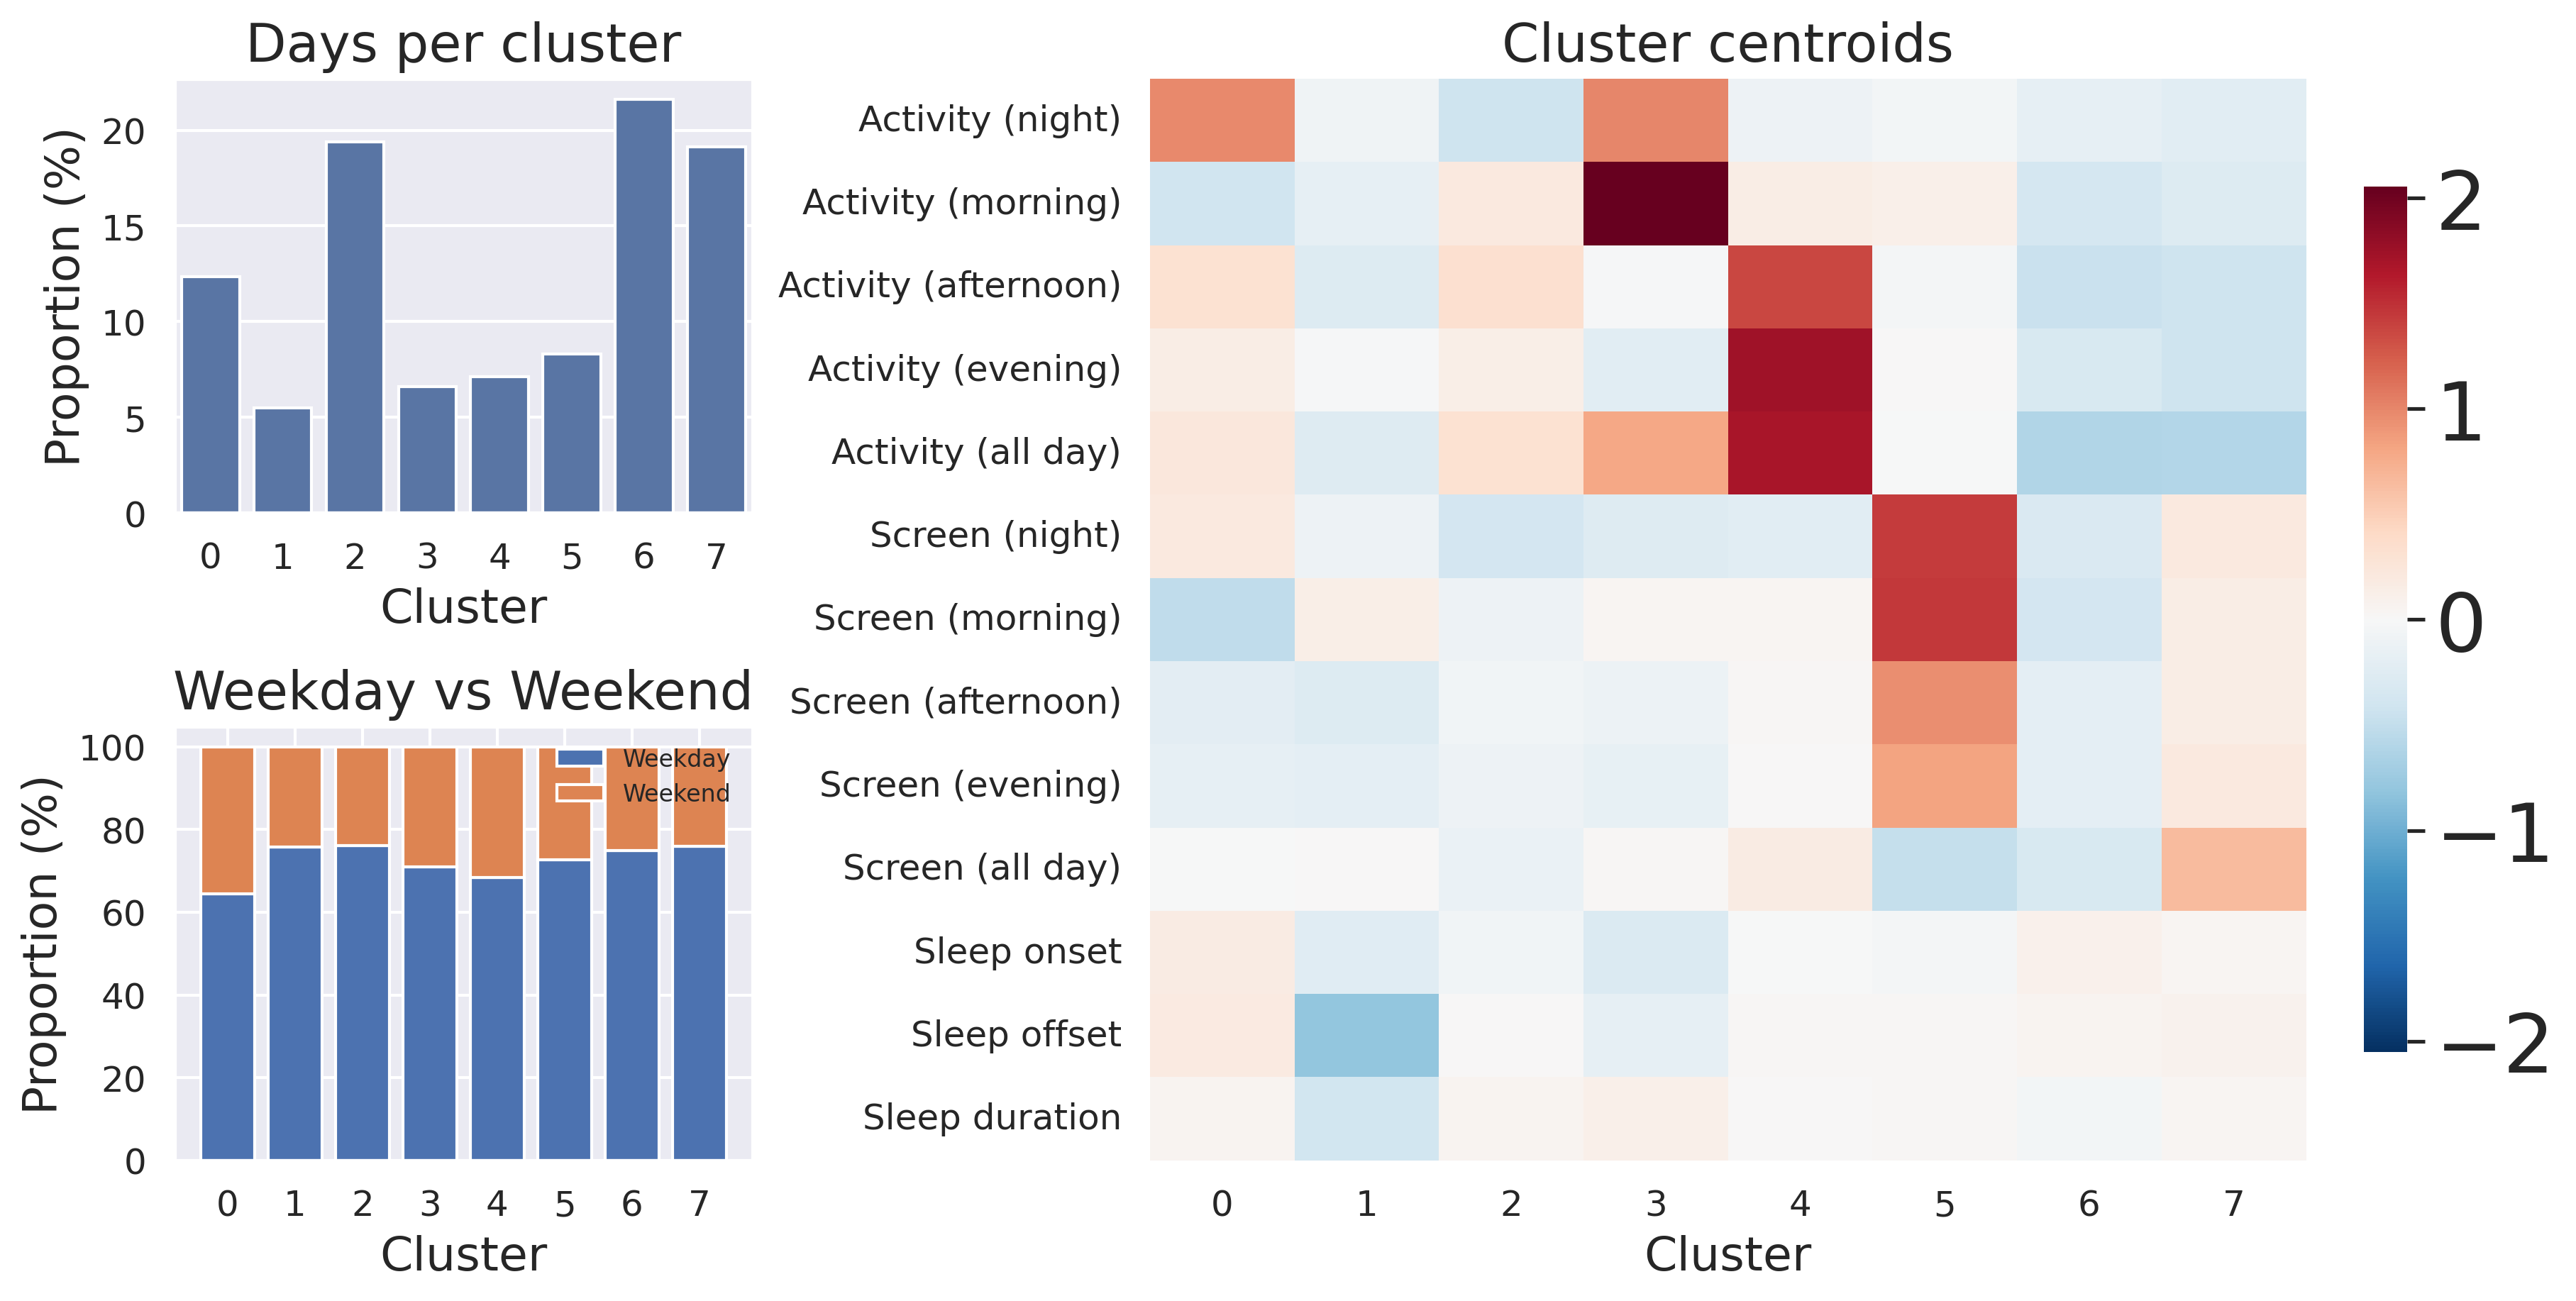
\includegraphics[width=\linewidth]{figures/appendix/globem_INS-W_3_summary.png}
    \caption{Cluster 3}
    \label{fig:globem_centroids_c}
  \end{subfigure}\hfill
  \begin{subfigure}[t]{0.485\textwidth}
    \centering
    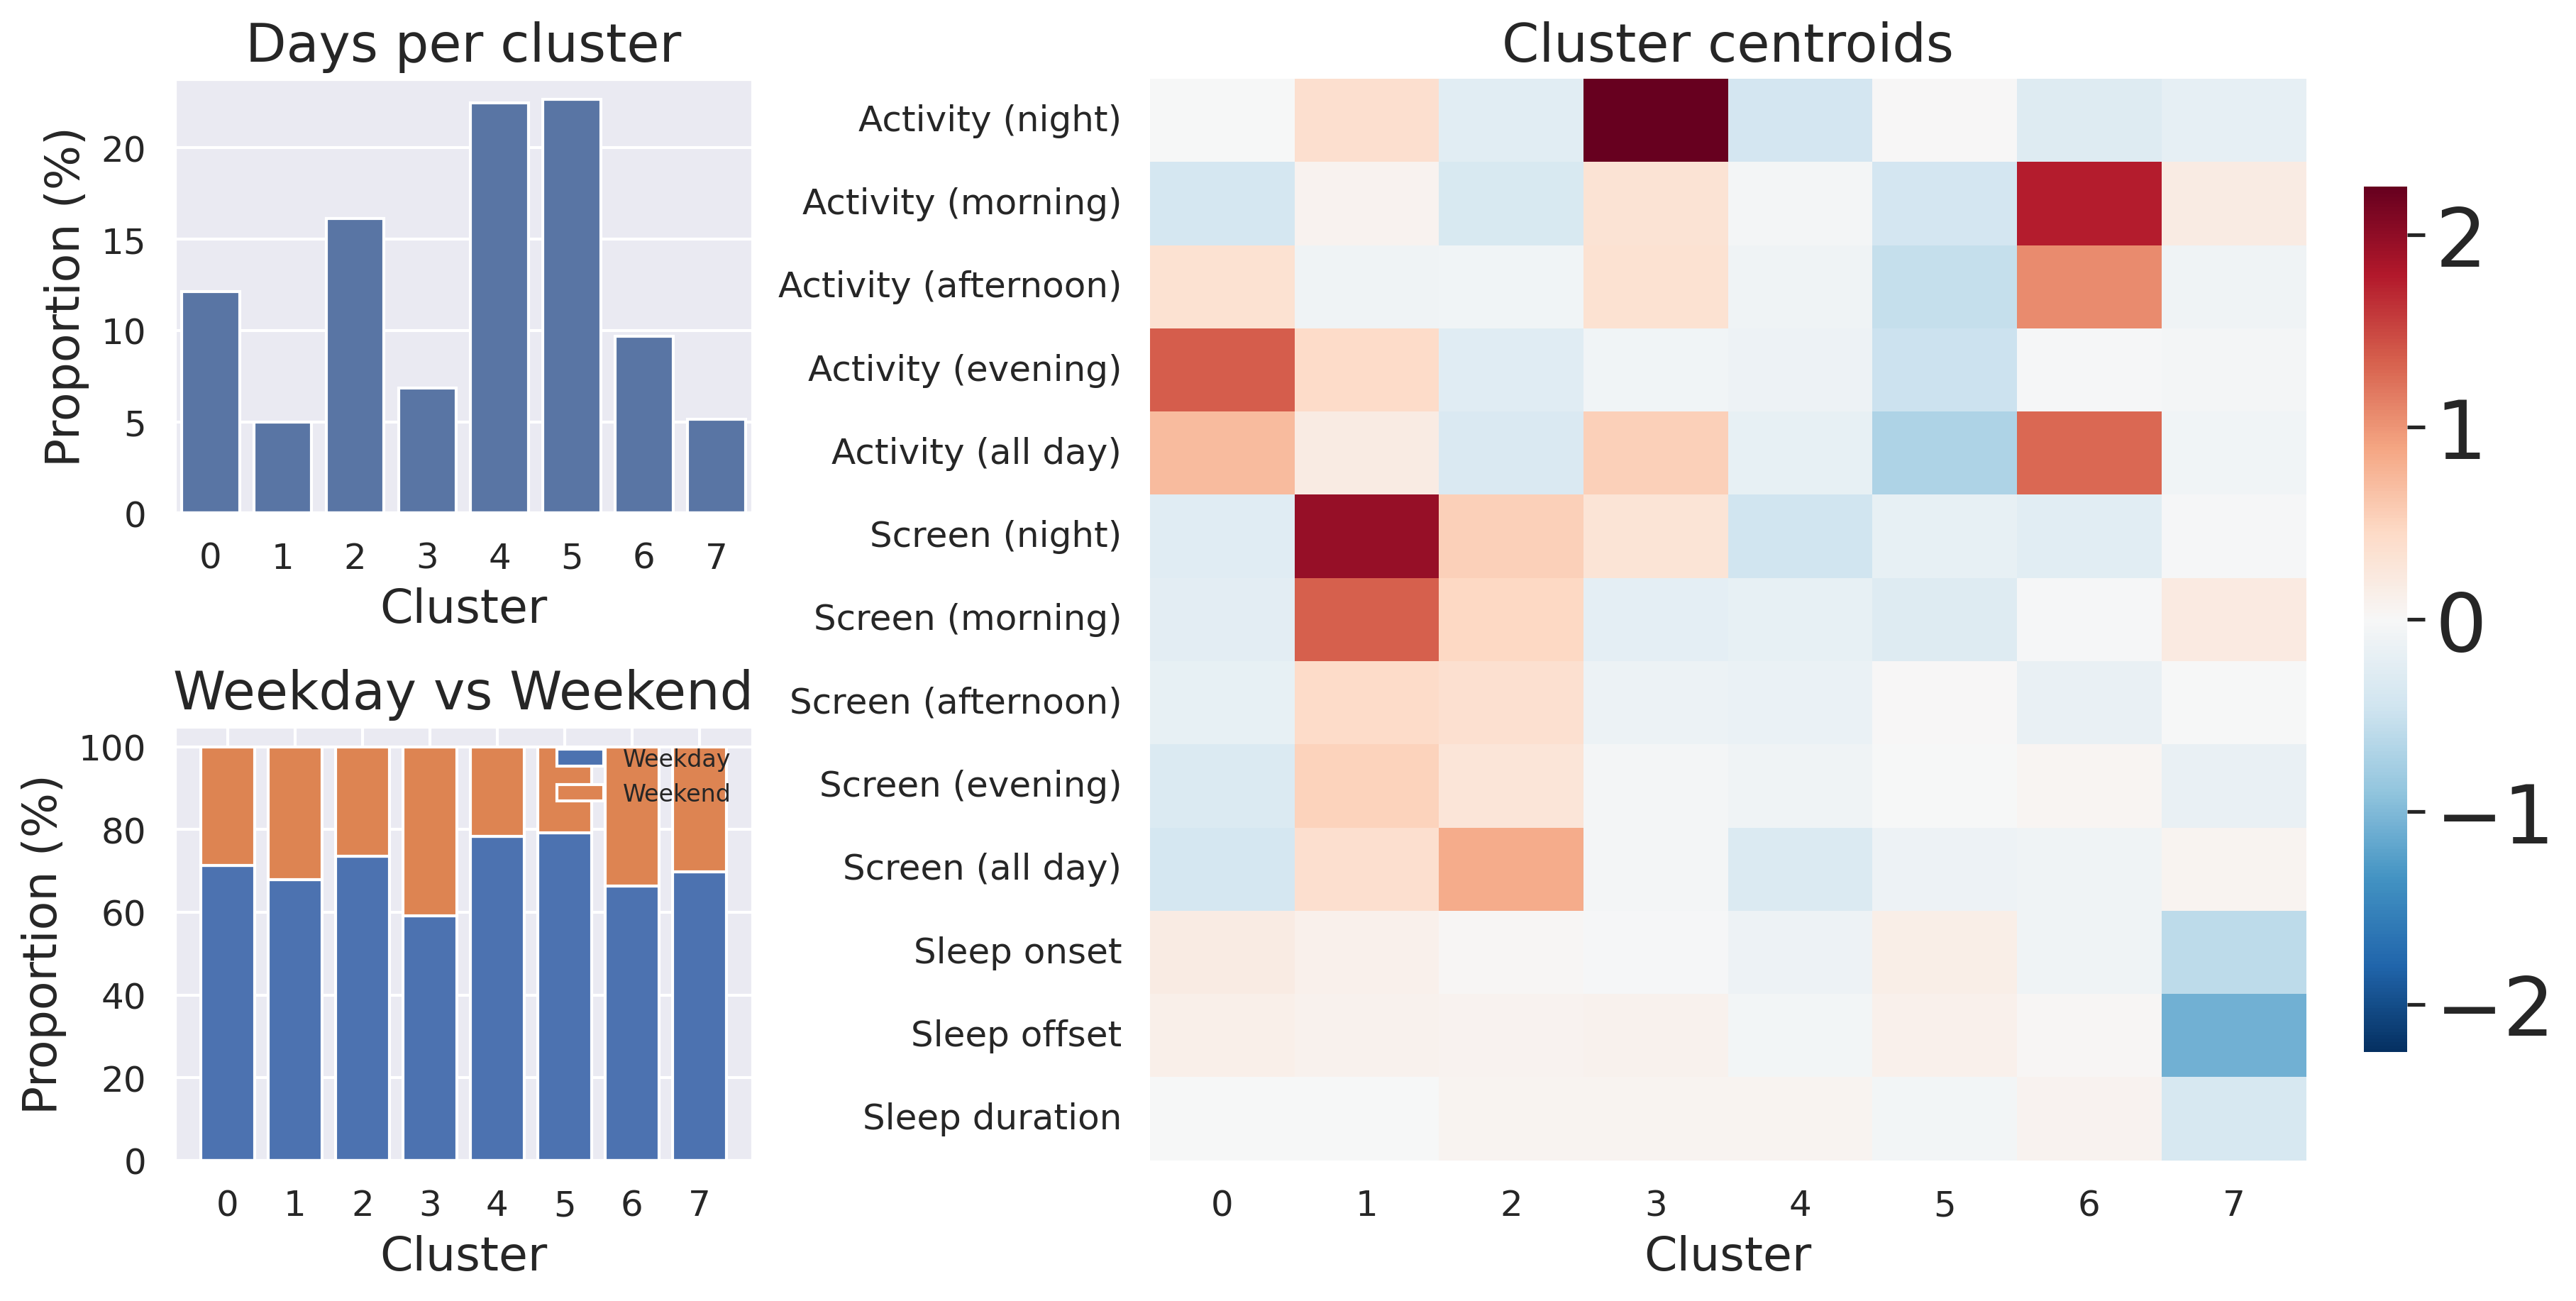
\includegraphics[width=\linewidth]{figures/appendix/globem_INS-W_4_summary.png}
    \caption{Cluster 4}
    \label{fig:globem_centroids_d}
  \end{subfigure}

  \caption{GLOBEM: Cluster centroid characteristics.}
  \label{fig:globem_centroids}
\end{figure}


% ---------- C: Signature with varying K ----------
\clearpage
\section{Signature with varying K components}

% (Add your figures/tables for this section here; using [p] + \FloatBarrier keeps them on this section’s pages.)

% \begin{figure}[p]
%   \centering
%   \includegraphics[width=\linewidth]{figures/appendix/signature_varying_K.png}
%   \caption{Signature stability under varying number of components K.}
%   \label{fig:signature_varying_K}
% \end{figure}
% \FloatBarrier

\end{appendices}


%%===========================================================================================%%
%% If you are submitting to one of the Nature Portfolio journals, using the eJP submission   %%
%% system, please include the references within the manuscript file itself. You may do this  %%
%% by copying the reference list from your .bbl file, paste it into the main manuscript .tex %%
%% file, and delete the associated \verb+\bibliography+ commands.                            %%
%%===========================================================================================%%

\bibliography{sn-bibliography}% common bib file
%% if required, the content of .bbl file can be included here once bbl is generated
%%\input sn-article.bbl


\end{document}
